\documentclass[nobib]{tufte-book}

\hypersetup{colorlinks}% uncomment this line if you prefer colored hyperlinks (e.g., for onscreen viewing)

%%
% Book metadata
\title{Notes on String Algorithms}
\subtitle{With Applications in Computational Biology}
\author{Kevin Gao}

%%
% If they're installed, use Bergamo and Chantilly from www.fontsite.com.
% They're clones of Bembo and Gill Sans, respectively.
%\IfFileExists{bergamo.sty}{\usepackage[osf]{bergamo}}{}% Bembo
%\IfFileExists{chantill.sty}{\usepackage{chantill}}{}% Gill Sans
%\usepackage{microtype}

\usepackage[square,numbers]{natbib}

%%
% Just some sample text
\usepackage{lipsum}

%%
% For nicely typeset tabular material
\usepackage{booktabs}

%%
% For graphics / images
\usepackage{graphicx}
\setkeys{Gin}{width=\linewidth,totalheight=\textheight,keepaspectratio}
\graphicspath{{figures/}}

% The fancyvrb package lets us customize the formatting of verbatim
% environments.  We use a slightly smaller font.
\usepackage{fancyvrb}
\fvset{fontsize=\normalsize}

%%
% Prints argument within hanging parentheses (i.e., parentheses that take
% up no horizontal space).  Useful in tabular environments.
\newcommand{\hangp}[1]{\makebox[0pt][r]{(}#1\makebox[0pt][l]{)}}

%%
% Prints an asterisk that takes up no horizontal space.
% Useful in tabular environments.
\newcommand{\hangstar}{\makebox[0pt][l]{*}}

%%
% Prints a trailing space in a smart way.
\usepackage{xspace}

%%
% For typesetting pseudocode
\usepackage{clrscode3e}

%%
% For typesetting math
\usepackage{amsmath}
\usepackage{amssymb}
\usepackage{amsthm}

%%
% For multiple columns typesetting
\usepackage{multicol}

\setcounter{tocdepth}{0}
\setcounter{secnumdepth}{0}
%%
% Theorem environments
\newtheorem{theorem}{Theorem}[chapter]
\newtheorem{lemma}[theorem]{Lemma}
\newtheorem{claim}[theorem]{Claim}
\newtheorem{corollary}[theorem]{Corollary}
\newtheorem{definition}[theorem]{Definition}
\newtheorem{rules}[theorem]{Rule}
\newtheorem{remark}[theorem]{Remark}
\newtheorem{example}[theorem]{Example}

% Prints the month name (e.g., January) and the year (e.g., 2008)
\newcommand{\monthyear}{%
  \ifcase\month\or January\or February\or March\or April\or May\or June\or
  July\or August\or September\or October\or November\or
  December\fi\space\number\year
}


% Prints an epigraph and speaker in sans serif, all-caps type.
\newcommand{\openepigraph}[2]{%
  %\sffamily\fontsize{14}{16}\selectfont
  \begin{fullwidth}
  \sffamily\large
  \begin{doublespace}
  \noindent\allcaps{#1}\\% epigraph
  \noindent\allcaps{#2}% author
  \end{doublespace}
  \end{fullwidth}
}

% Inserts a blank page
\newcommand{\blankpage}{\newpage\hbox{}\thispagestyle{empty}\newpage}

\usepackage{units}

% Typesets the font size, leading, and measure in the form of 10/12x26 pc.
\newcommand{\measure}[3]{#1/#2$\times$\unit[#3]{pc}}

% Macros for typesetting the documentation
\newcommand{\hlred}[1]{\textcolor{Maroon}{#1}}% prints in red
\newcommand{\hangleft}[1]{\makebox[0pt][r]{#1}}
\newcommand{\hairsp}{\hspace{1pt}}% hair space
\newcommand{\hquad}{\hskip0.5em\relax}% half quad space
\newcommand{\TODO}{\textcolor{red}{\bf TODO!}\xspace}
\newcommand{\na}{\quad--}% used in tables for N/A cells
\providecommand{\XeLaTeX}{X\lower.5ex\hbox{\kern-0.15em\reflectbox{E}}\kern-0.1em\LaTeX}
\newcommand{\tXeLaTeX}{\XeLaTeX\index{XeLaTeX@\protect\XeLaTeX}}
% \index{\texttt{\textbackslash xyz}@\hangleft{\texttt{\textbackslash}}\texttt{xyz}}
\newcommand{\tuftebs}{\symbol{'134}}% a backslash in tt type in OT1/T1
\newcommand{\doccmdnoindex}[2][]{\texttt{\tuftebs#2}}% command name -- adds backslash automatically (and doesn't add cmd to the index)
\newcommand{\doccmddef}[2][]{%
  \hlred{\texttt{\tuftebs#2}}\label{cmd:#2}%
  \ifthenelse{\isempty{#1}}%
    {% add the command to the index
      \index{#2 command@\protect\hangleft{\texttt{\tuftebs}}\texttt{#2}}% command name
    }%
    {% add the command and package to the index
      \index{#2 command@\protect\hangleft{\texttt{\tuftebs}}\texttt{#2} (\texttt{#1} package)}% command name
      \index{#1 package@\texttt{#1} package}\index{packages!#1@\texttt{#1}}% package name
    }%
}% command name -- adds backslash automatically
\newcommand{\doccmd}[2][]{%
  \texttt{\tuftebs#2}%
  \ifthenelse{\isempty{#1}}%
    {% add the command to the index
      \index{#2 command@\protect\hangleft{\texttt{\tuftebs}}\texttt{#2}}% command name
    }%
    {% add the command and package to the index
      \index{#2 command@\protect\hangleft{\texttt{\tuftebs}}\texttt{#2} (\texttt{#1} package)}% command name
      \index{#1 package@\texttt{#1} package}\index{packages!#1@\texttt{#1}}% package name
    }%
}% command name -- adds backslash automatically
\newcommand{\docopt}[1]{\ensuremath{\langle}\textrm{\textit{#1}}\ensuremath{\rangle}}% optional command argument
\newcommand{\docarg}[1]{\textrm{\textit{#1}}}% (required) command argument
\newenvironment{docspec}{\begin{quotation}\ttfamily\parskip0pt\parindent0pt\ignorespaces}{\end{quotation}}% command specification environment
\newcommand{\docenv}[1]{\texttt{#1}\index{#1 environment@\texttt{#1} environment}\index{environments!#1@\texttt{#1}}}% environment name
\newcommand{\docenvdef}[1]{\hlred{\texttt{#1}}\label{env:#1}\index{#1 environment@\texttt{#1} environment}\index{environments!#1@\texttt{#1}}}% environment name
\newcommand{\docpkg}[1]{\texttt{#1}\index{#1 package@\texttt{#1} package}\index{packages!#1@\texttt{#1}}}% package name
\newcommand{\doccls}[1]{\texttt{#1}}% document class name
\newcommand{\docclsopt}[1]{\texttt{#1}\index{#1 class option@\texttt{#1} class option}\index{class options!#1@\texttt{#1}}}% document class option name
\newcommand{\docclsoptdef}[1]{\hlred{\texttt{#1}}\label{clsopt:#1}\index{#1 class option@\texttt{#1} class option}\index{class options!#1@\texttt{#1}}}% document class option name defined
\newcommand{\docmsg}[2]{\bigskip\begin{fullwidth}\noindent\ttfamily#1\end{fullwidth}\medskip\par\noindent#2}
\newcommand{\docfilehook}[2]{\texttt{#1}\index{file hooks!#2}\index{#1@\texttt{#1}}}
\newcommand{\doccounter}[1]{\texttt{#1}\index{#1 counter@\texttt{#1} counter}}

\newcommand{\N}{\mathbb{N}}
\newcommand{\Z}{\mathbb{Z}}

% Generates the index
\usepackage{makeidx}
\makeindex


\titlecontents{part}
    [0pt]
    {\addvspace{0.25\baselineskip}}
    {{Part~\thecontentslabel}}
    {{Part~\thecontentslabel}}
    {}
    [\vspace*{0.5\baselineskip}]

\titlecontents{chapter}
    [4em]
    {}
    {\contentslabel{2em}\textit}
    {\hspace{0em}\textit}
    {\qquad\thecontentspage}
    [\vspace*{0.5\baselineskip}]

\begin{document}

% Front matter
\frontmatter

% r.1 blank page

% v.2 epigraphs

% r.3 full title page
\maketitle


% v.4 copyright page
\newpage
\begin{fullwidth}
~\vfill
\thispagestyle{empty}
\setlength{\parindent}{0pt}
\setlength{\parskip}{\baselineskip}
Copyright \copyright\ \the\year\ \thanklessauthor

\par\smallcaps{terra-incognita.dev}

\par Licensed under the Apache License, Version 2.0 (the ``License''); you may not
use this file except in compliance with the License. You may obtain a copy
of the License at \url{http://www.apache.org/licenses/LICENSE-2.0}. Unless
required by applicable law or agreed to in writing, software distributed
under the License is distributed on an \smallcaps{``AS IS'' BASIS, WITHOUT
WARRANTIES OR CONDITIONS OF ANY KIND}, either express or implied. See the
License for the specific language governing permissions and limitations
under the License.


\end{fullwidth}

% r.5 contents
\tableofcontents

% r.7 dedication
\cleardoublepage
~\vfill

{\noindent\fontsize{18}{22}\selectfont\itshape
These notes are primarily based on the book \textbf{Algorithms on Strings, Trees, and Sequences} by \textbf{Dan Gusfield} \cite{gusfield_1997}.

\hfill

\noindent Thanks Professor Gusfield for his great book.

\hfill

The part on indexing and compression is based on the book \textbf{Genome-Scale Algorithm Design} \cite{makinen_belazzougui_cunial_tomescu_2015} and Ben Langmead's lectures.
}

\vfill
\vfill


% r.9 introduction
\cleardoublepage


%%
% Start the main matter (normal chapters)
\mainmatter

\part{Comparison-Based Exact Matching}

\chapter{Naive Exact Matching}
(Gusfield Section 1.1)

\newthought{Terminology Confusion}. Before starting the discussion of string matching algorithms, we should note the difference between a \textit{\textbf{substring}} and a \textit{\textbf{subsequence}}. Given a string S, characters in a substring of S must occur contiguously in S; whereas characters in a subse- quence may be interspersed gaps (or indels, as we call them in biology) and/or characters not in the original string.

\section{Exact String Mathching Problem}

Given a text string $T$ and pattern $P$, the goal of the exact string matching problem is to find all occurrences of $P$ in $T$.

\section{The ``Na\"ive'' Algorithm} \index{naive exact matching algorithm}

\begin{codebox}
    \Procname{$\proc{Naive-Match}(P,T)$}
    \li $\id{matches} = [\;]$
    \li \For $i=1$ \To $|T|-|P|+1$ \Do
        \li $\id{match} = \const{true}$
        \li \For $j = 1$ \To $|P|$ \Do
            \li \If $T[i+j] \neq P[j]$ \Then
                \li $\id{match} = \const{false}$
                \li \textbf{break}
            \End
        \li \If $\id{match}$ \Then
            \li $\id{matches}.\proc{Append}(i)$ 
        \End
    \End
    \li \Return $\id{matches}$ 
\end{codebox}

\begin{marginfigure}
    \caption{Naive exact matching with $P=abxyabxa$ and $T=xabxyabxyabxz$.}
    \begin{alignat*}{7}
        T:\; &x&&a&&b&&x&&y&&abxyabxz \\
        P:\; &a&&b&&x&&y&&a&&bxa \\
        & && a&&b&&x&&y&&abxa \\
        & && && a&&b&&x&&yabxa \\
        & && && && a&&b&&xyabxa \\
        & && && && && a &&bxyabxa \\
        & && && && && && abxyabxa \\
    \end{alignat*}
    \label{fig:naive-matching}
\end{marginfigure}

The na\"ive exact matching algorithm aligns the left end of $P$ with the left end of $T$ and compares the characters of $P$ and $T$ left to right until a mismatch is found, or until it reaches the end of $P$, in which case we report the position of $P$. Then, $P$ is shifted to the right by one place. We repeat this procedure until the right end of $P$ passes the right end of $T$.

\section{Runtime of the Naive Algorithm}

Let $n = |P|$ and $m = |T|$. The worst-case comparisons made by the naive algorithm is $\Theta(nm)$. We have the lower bound $\Omega(nm)$ when
$P$ and $T$ contains the same repeated characters (e.g. $P = aaa$, $T = aaaaaaaaa$), in which case the algorithm makes $n(m-n+1) \in \Omega(nm)$ comparisons.

\chapter{Z Algorithm}
(Gusfield Chapter 1)

\section{Speeding Up the Naive Algorithm}

The naive exact matching algorithm is stupid. It always shifts $P$ by only one even if it knows for sure that the next shift will not yield a match. This gives us some ideas on how to improve the algorithm. If we can shift $P$ by more than one character, but never shift so far as to miss the next occurrence of $P$ in $T$, we can improve the runtime of the naive algorithm.

Doing this, however, requires us to have some prior knowledge of the pattern $P$ or the text $T$.

\section{Foundamental Preprocessing}

A fundemental preprocessing is a generalized way to process the pattern $P$ to gain knowledge of the pattern, independent of any particular algorithm.

\begin{definition}
    Given a string $S$ and a position $i>1$, let $Z_i(S)$ be the length of the longest substring of $S$ that starts at $i$ and matches a prefix of $S$.

    In other words, $Z_i(S)$ is the length of the longest prefix of $S[i\ldots |S|]$ that matches a prefix of $S$.
\end{definition}

\begin{definition}[Z-box] \index{Z-box}
    For any position $i > 1$ where $Z_i$ is greater than 0, the \textbf{Z-box} at $i$ is the interval starting at $i$ and ending at $i+Z_i-1$.
\end{definition}

\begin{marginfigure}
    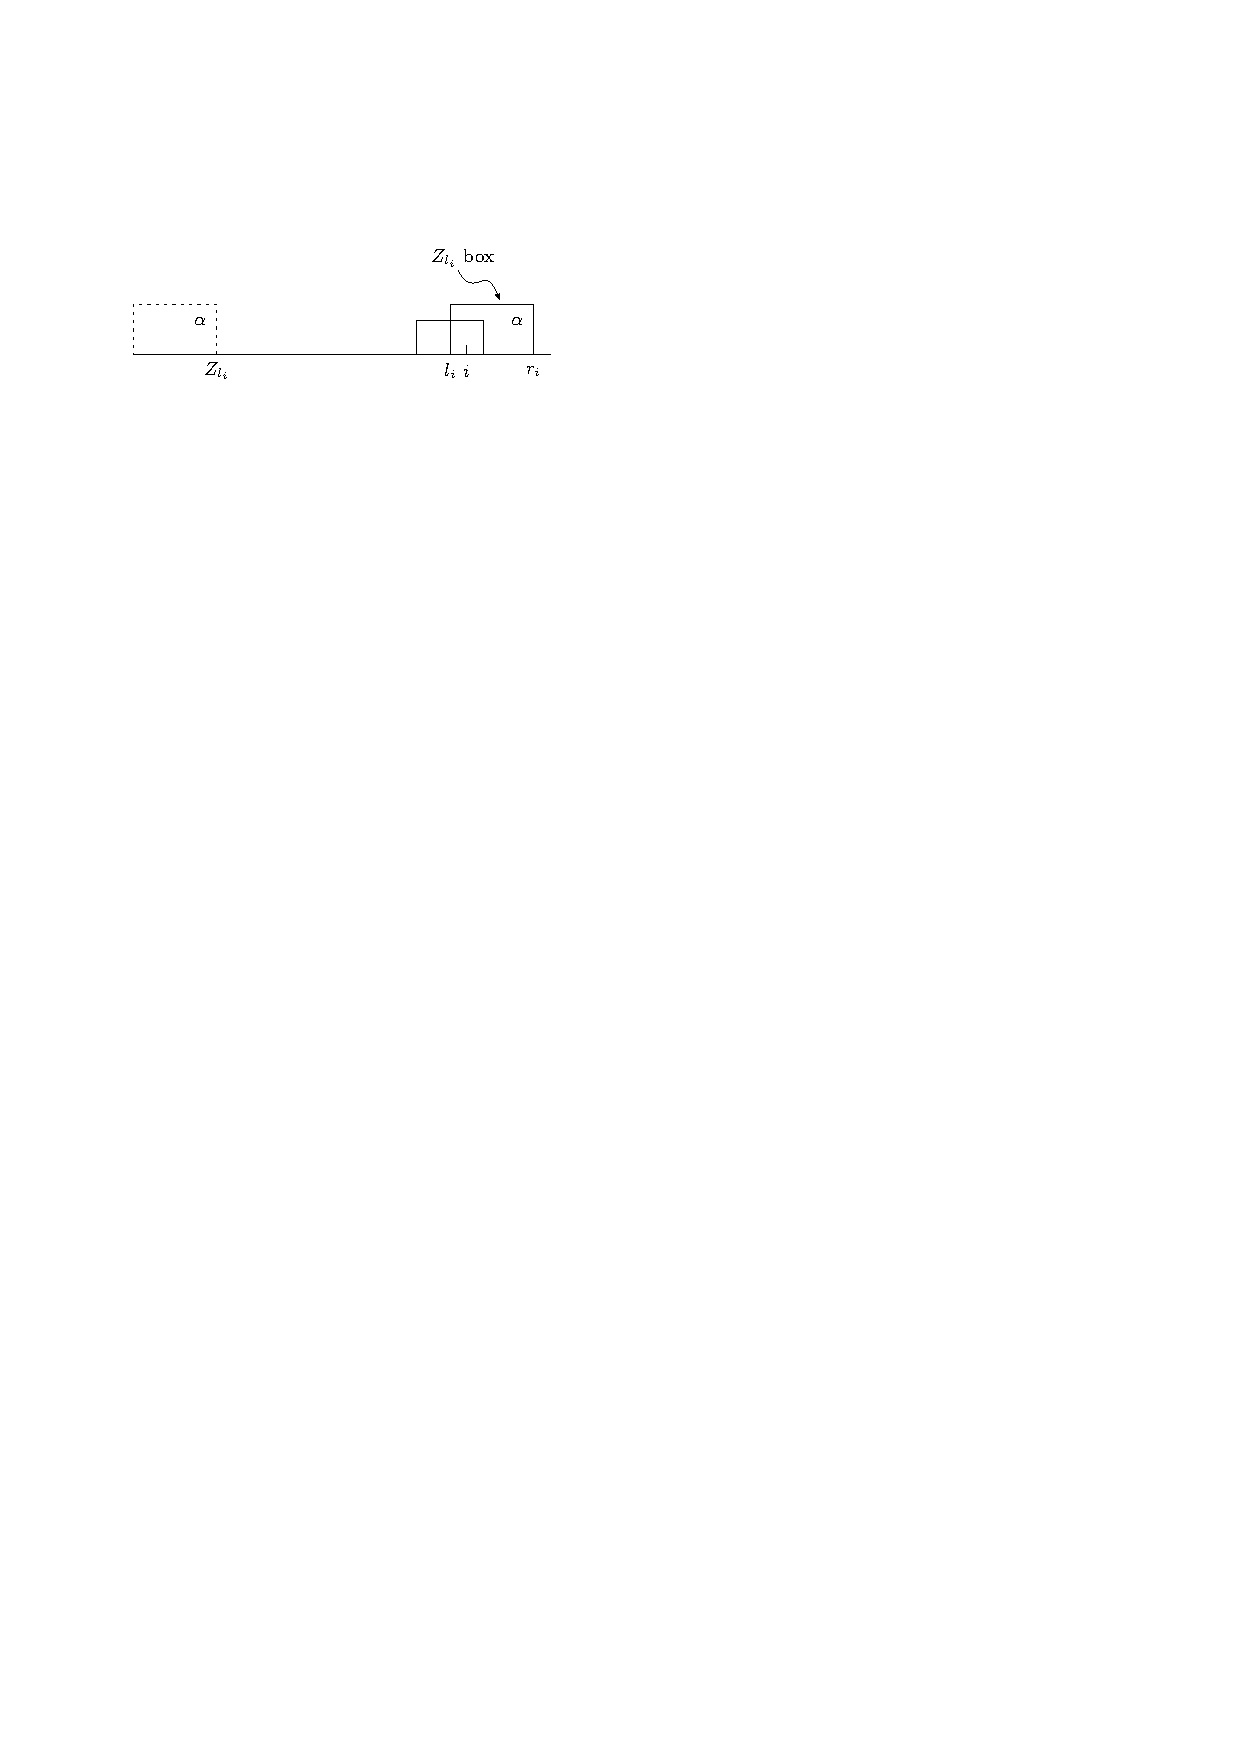
\includegraphics[width=\linewidth]{z/z-box.pdf}
    \caption{Relations between $i$, $l_i$, $r_i$ and the Z-box at $l_i$.}
    \label{fig:z-box}
\end{marginfigure}

\begin{definition}
    For every $i > 1$, $r_i$ is the right endpoint of the Z-box that begins at or befor position $i$ (i.e. the closest Z-box to the left). More formally, $r_i$ is the largest value of $j + Z_j - 1$ over all $1 < j \leq i$ such that $Z_j > 0$.
\end{definition}

\index{fundamental preprocessing}
The linear-time computation of the $Z_i$ values for all $i \in \{1,\ldots,|S|\}$ from the string $S$ is called the \textit{\textbf{fundamental preprocessing}} task.

\section{The Z Algorithm} \index{Z algorithm}

The \textit{\textbf{Z algorithm}} is an algorithm for computing the fundamental preprocessing. The Z algorithm is similar to a dynamic programming algorithm in the sense that it uses memoized information to speed up the computation and reduce the number of comparison needed. Namely, assume there exists $j < i$ such that $j + Z[j] - 1 > i$, then we can use $Z[i-j+1]$ to infer $Z[i]$.

\begin{figure}[htbp]
    \centering
    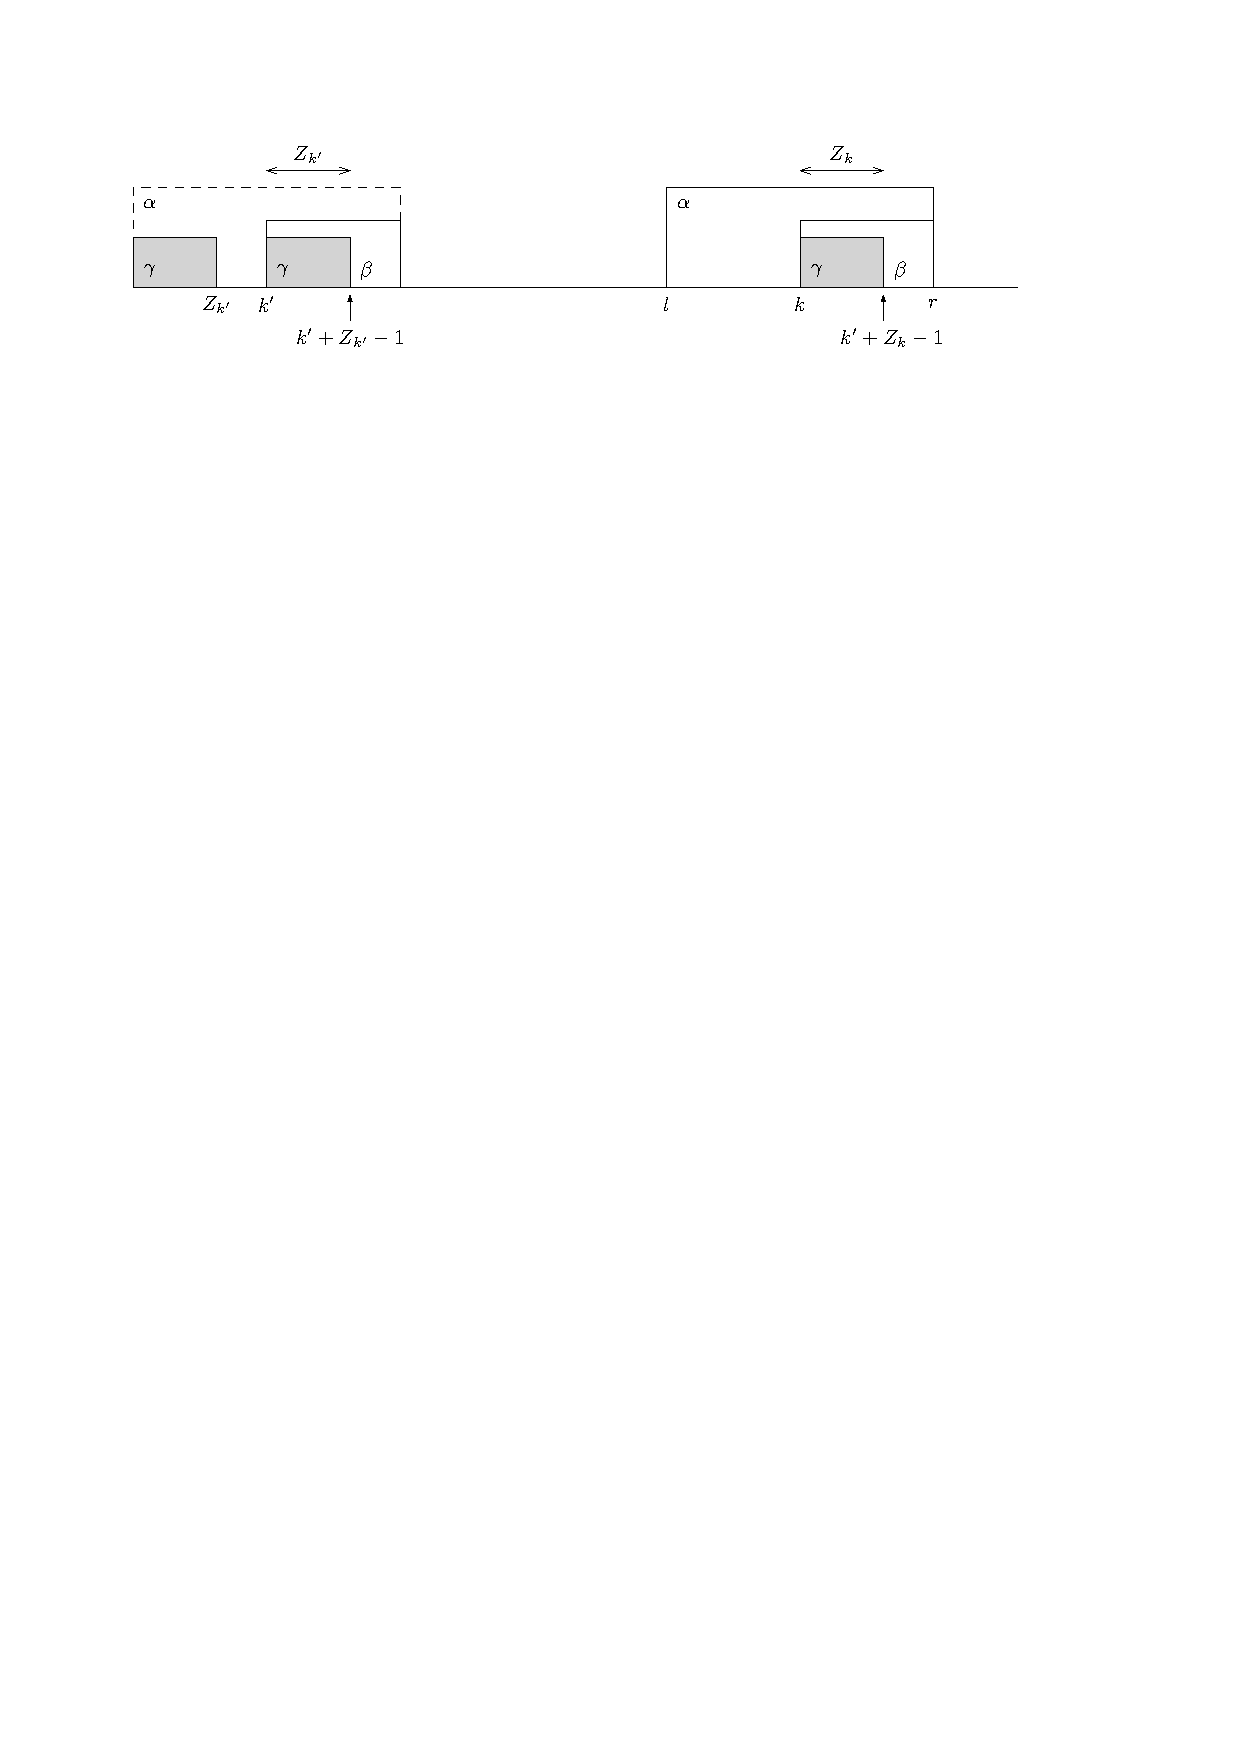
\includegraphics[width=\linewidth]{z/z-process-case2a.pdf}
    \caption{Case 2a: The longest string starting at $k'$ that matches a prefix of $S$ is shorter than $|\beta| = r-k+1$. In this case, $Z_k = Z_{k'}$.}
    \label{fig:z-process-case2a}
\end{figure}

\begin{figure}[htbp]
    \centering
    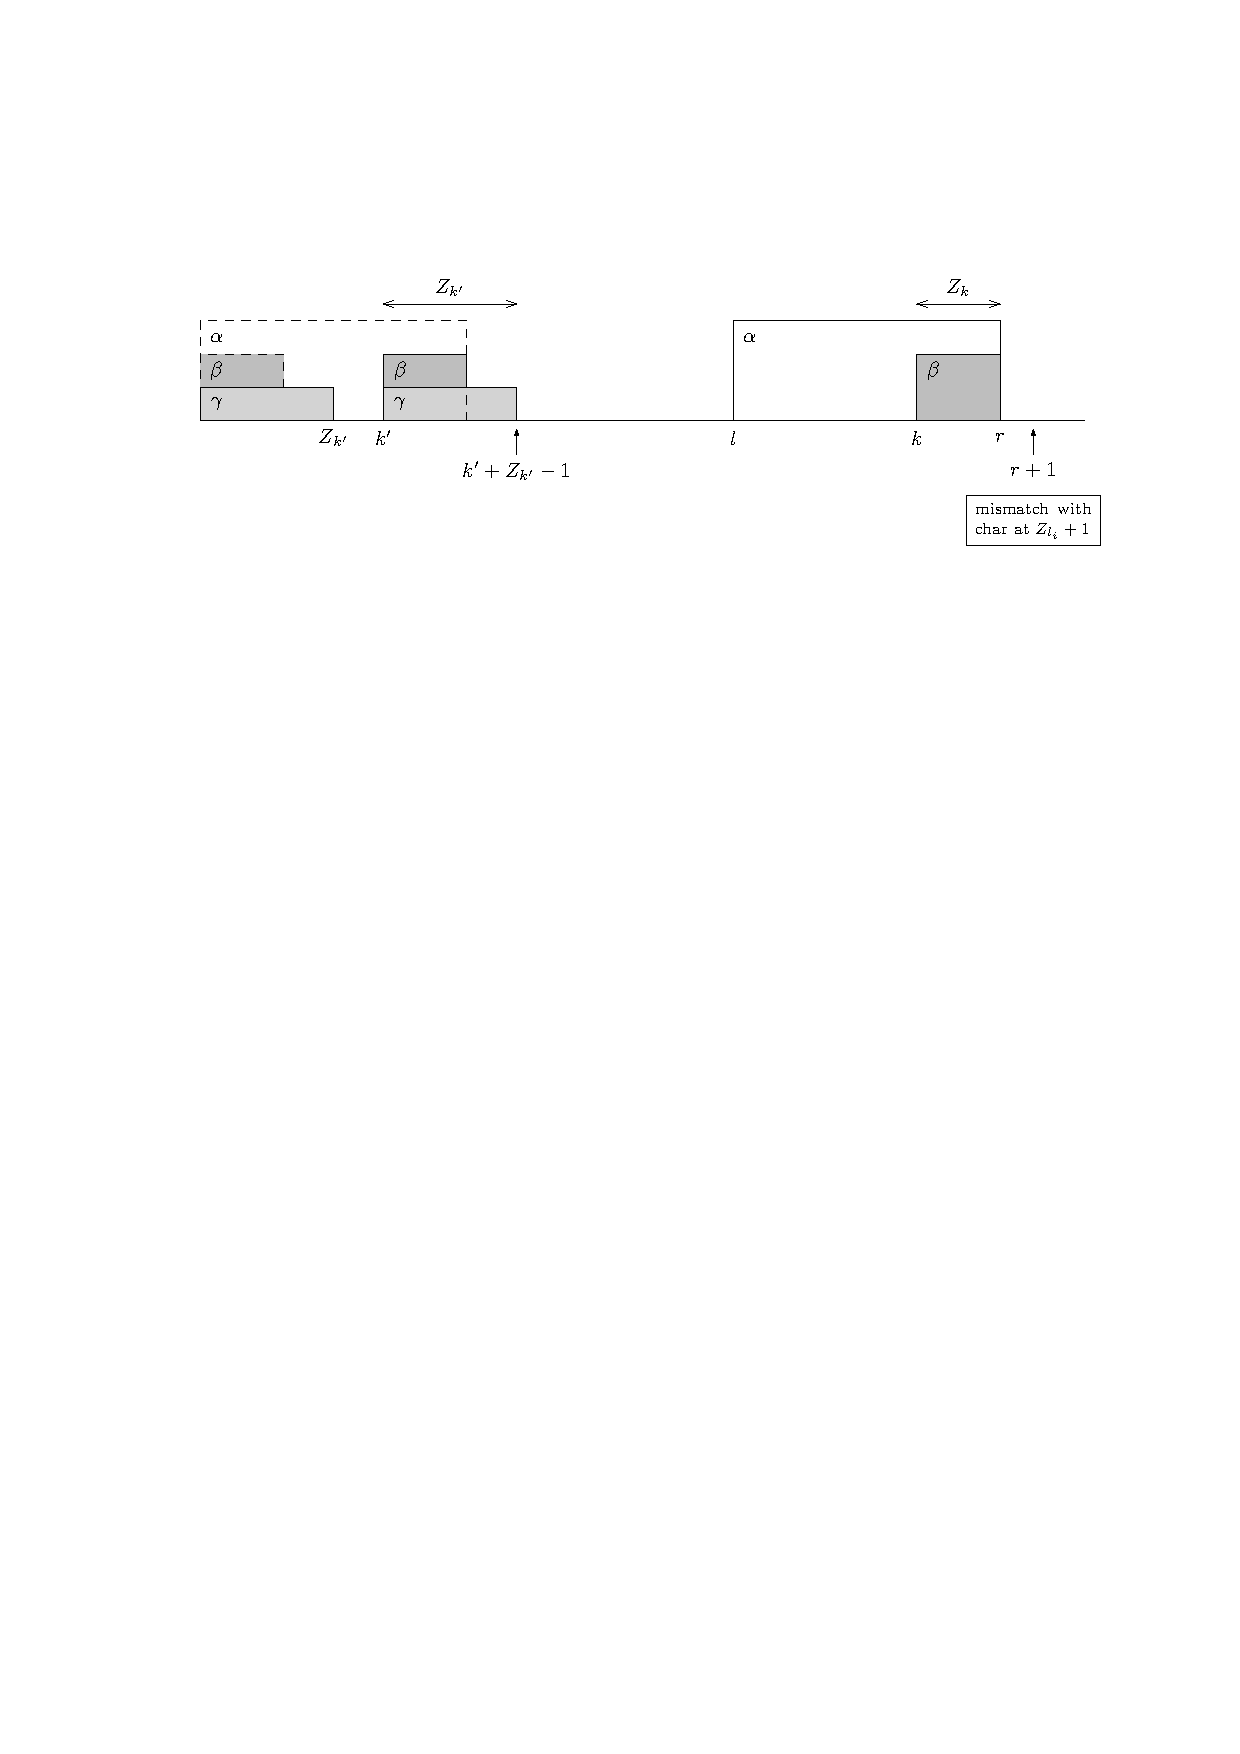
\includegraphics[width=\linewidth]{z/z-process-case2b1.pdf}
    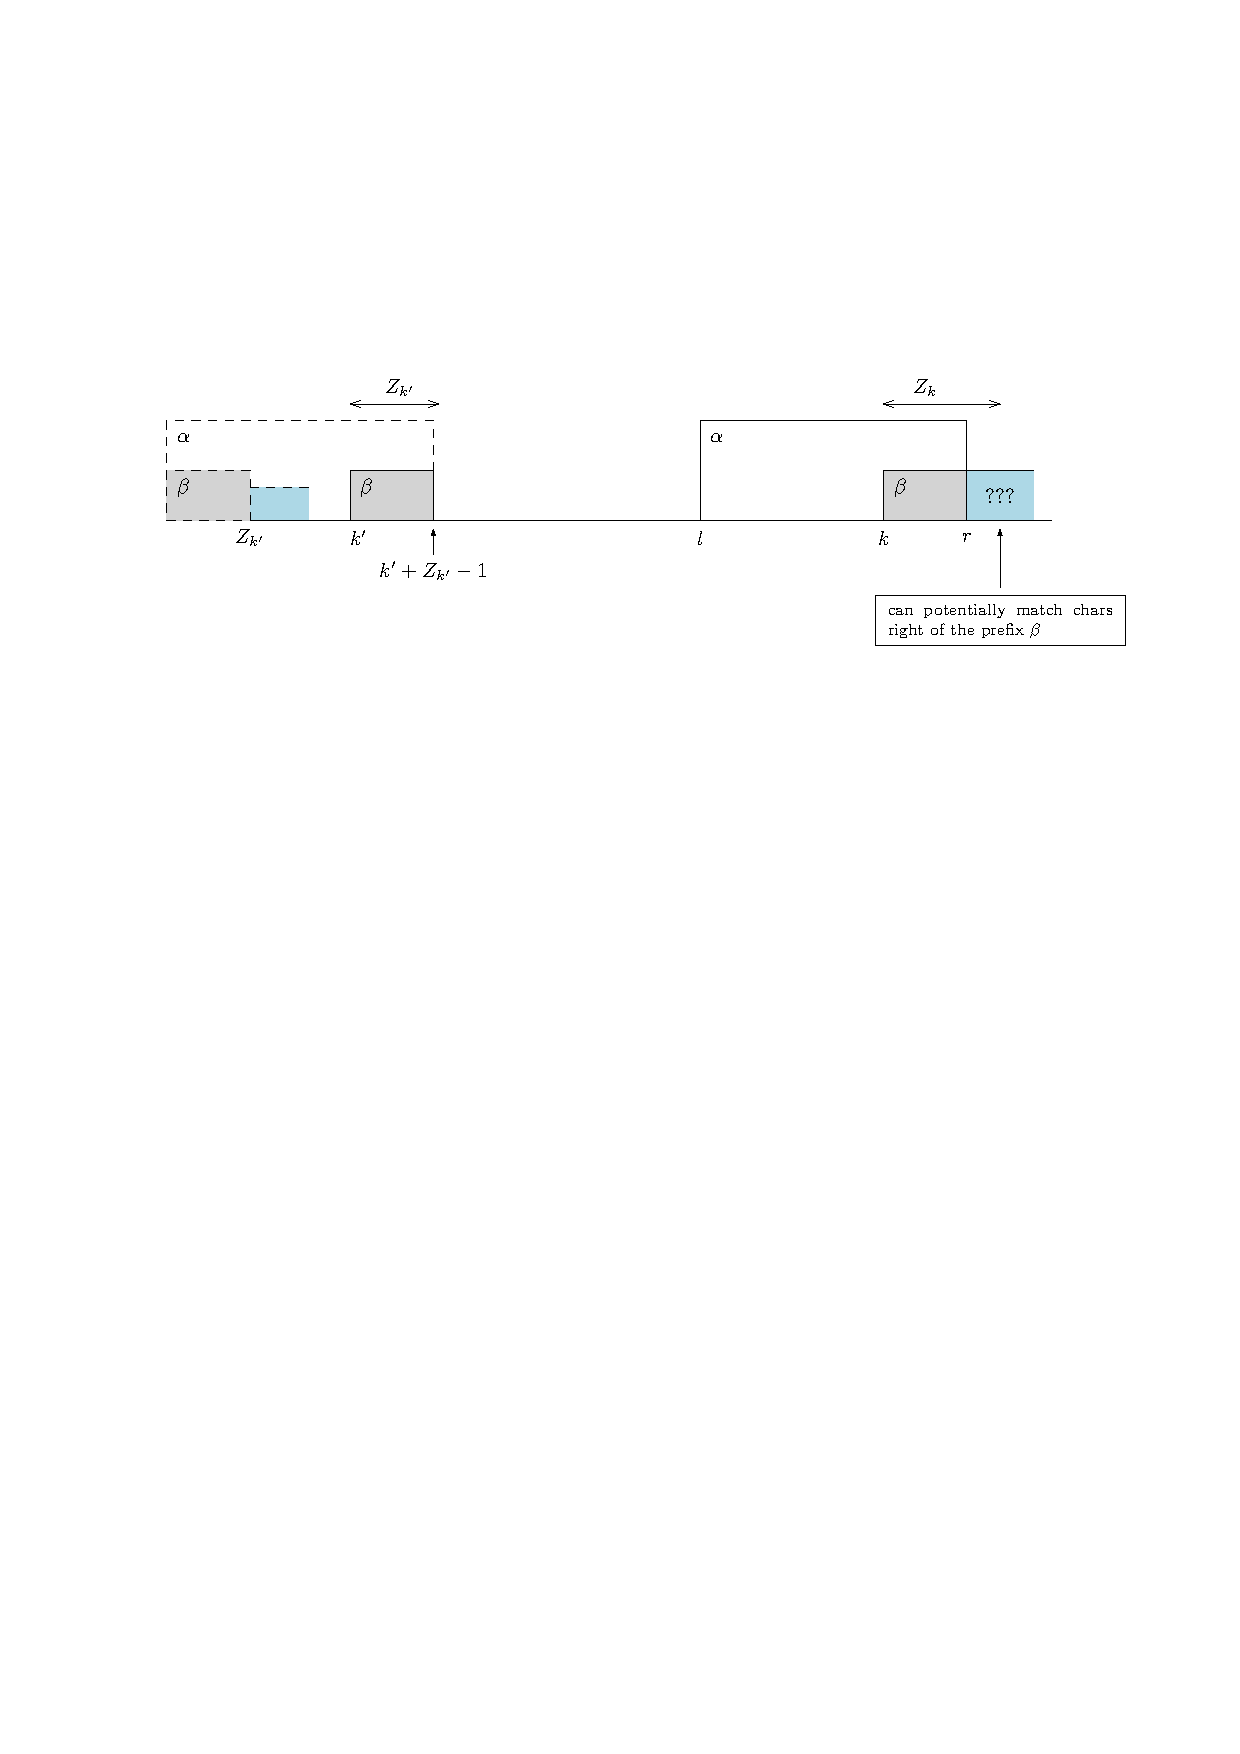
\includegraphics[width=\linewidth]{z/z-process-case2b2.pdf}
    \caption{Case 2b: The longest string starting at $k'$ that matches a prefix of $S$ is at least $|\beta| = r-k+1$. In this case, we continue to compare characters right of $r$ with characters right of the $Z_{k'}$th character until mismatch. }
    \label{fig:z-process-case2b}
\end{figure}

Given $Z_i$ for all $1 < i \leq k-1$ and the current $l$ and $r$, we can compute $Z_k$ using the following procedure:

\begin{enumerate}
    \item Case 1: If $k > r$, $k$ is not in an existing Z-box. Compute $Z_k$ by explicitly comparing each character starting at $k$ with prefix of $S$.
    \item Case 2: If $k \leq r$, $k$ is in an existing Z-box, denoted $\alpha$, that matches a prefix of $S$. Hence, character $S[k]$ also appears in the prefix at position $k' = k - l + 1$. \\ We also consider the substring $S[k\ldots r]$, denoted $\beta$. By the same reasoning, $\beta$ matches the substring $S[k'\ldots Z_l]$.
    \begin{enumerate}
        \item $Z_{k'} < |\beta|$. This implies that the longest string starting at $k'$ that matches a prefix of $S$, $\gamma$, is shorter $|\beta|$. Then, $Z_{k} = Z_{k'}$, and $l,r$ remain unchanged. Note that $|\gamma|$ can be 0.
        \item $Z_{k'} \geq |\beta|$. This means $S[k\ldots r]$ is at least a prefix of $S$. However, $Z_k$ might be larger than $|\beta|$. We cannot determine this solely based on the existing information as characters beyond the $Z_l$th character are not included in $\alpha$. So, we compare the characters starting at position $r+1$ of $S$ to the characters starting at position $|\beta|+1$ of $S$, until a mismatch occurs. Say the mismatch occur at position $q$. Then, $Z_k = q- k$, $r = q-1$, and $l = k$. (If $Z_{k'} > |\beta|$, a mismatch occurs immediate after the $Z_{l}$th character because otherwise, the $(r+1)$th character matches the $Z_{l}$th character, and we would have a longer $\alpha$ and a larger $Z_l$)
    \end{enumerate}
\end{enumerate}

\begin{codebox}
    \Procname{$\proc{Compute-Z}(S)$}
    \li $n = |S|$
    \li $l,r,k = 1$
    \li $Z = \text{empty array of length $n$}$
    \li \For $k=2$ \To $n$ \Do
        \li \If $k > r$ \Then \RComment{Case 1}
            \li \Comment{compute $Z[k]$ from scratch}
            \li $l,r = k$ 
            \li \While $r \leq n$ \textbf{and} $S[r-l+1] \isequal S[r]$ \Do
                \li $r = r + 1$
            \End
            \li $Z[k] = r-l$
            \li $r = r - 1$
        \li \Else \RComment{Case 2}
            \li $k' = k - l + 1$
            \li \If $Z[k'] < r - k + 1$ \Then \RComment{Case 2a}
                \li $Z[k] = Z[k']$ 
            \li \Else \RComment{Case 2b}
                \li $q = r+1$
                \li \While $q \leq n$ \textbf{and} $S[q-l + 1] \isequal S[q]$ \Do
                    \li $q = q + 1$
                \End
                \li $Z[k] = q-k$
                \li $l,r = k, \,q-1$ 
            \End
        \End
        \End
        \li \Return $Z$ 
\end{codebox}

For a step-by-step animation of the Z algorithm, see \\
\href{https://personal.utdallas.edu/~besp/demo/John2010/z-algorithm.htm}{https://personal.utdallas.edu/\textasciitilde besp/demo/John2010/z-algorithm.htm}

\section{Running Time of the Z Algorithm}

\begin{theorem}
    All the $Z_i$ values can be computed by the Z algorithm with at most $2|S| \in O(|S|)$ comparisons.
\end{theorem}

\begin{proof}
    The time is proportional to the number of iterations, $|S|$, plus the number of character comparisons.
    
    Each iteration that does any character comparison ends as soon as there is a mismatch, so there are at most $|S|$ \textbf{mismatches}. In every iteration where there is a match, $r$ moves to the right by an amount at least as large as the number of matches. This implies that there are at most $|S|$ \textbf{matches}. Note that once a character results in a match, it is not compared again.

    Every character comparison is either a match or mismatch, so the total number of comparisons is at most $2|S|$.
\end{proof}

\section{Correctness of the Z Algorithm}

\begin{theorem}
    At the $k$th iteration of the algorithm, \proc{Compute-Z} correctly calculates $Z_k$, and $l,r$ are updated correctly.
\end{theorem}

\begin{proof}
    By a case analysis.

    Case 1: Trivial since it's just explicit comparison.

    Case 2a: We claim that the substring at position $k$ can match a prefix of $S$ only for length $Z_{k'} < |\beta|$. Prove the claim by contradiction (suppose not, we would have a longer prefix matching the substring at $k'$, contradicting the maximality of $Z_{k'}$).

    Case 2b: $\beta$ must be a prefix of $S$ as established above. Characters beyond $r$ are explicitly compared.
\end{proof}

\begin{corollary}
    \proc{Compute-Z} correctly calculates $Z_k$ for all $k \in \{2,\ldots,|S|\}$.
\end{corollary}

\begin{proof}
    By induction on $k$.
\end{proof}

\section{Z Algorithm for Exact Matching}

The Z algorithm lends itself to a linear-time algorithm for exact matching. Given a pattern $P$ and text $T$, we construct a new string $P \$ T$ where $\$$ is a \textit{\textbf{separator}} (a.k.a. \textit{\textbf{delimiter}} or \textit{\textbf{sentinel}}) such that $\$ \not\in \Sigma$. We construct the Z-array for this new string. It takes $O(|P|+|T|)$ time to construct the Z-array. After this, we can simply make a pass through the Z-array and read the result from it. This takes $O(|T|)$ time.

\begin{codebox}
    \Procname{$\proc{Z-Exact-Matching}(P,T)$}
    \li $\id{query} = P + ``\$" + T$
    \li $Z = \proc{Compute-Z}(\id{query})$
    \li \For $i = |P|+1$ \To $|P|+|T|+1$ \Do
        \li \If $Z[i] \isequal |P|$ \Then
            \li pattern found at index $i - |P|$ 
\end{codebox}

\chapter{Boyer-Moore}
(Gusfield Chapter 2)

\newthought{Key Ideas} of the Boyer-Moore algorithm: right-to-left scan, bad character rule, good suffix rule.

\section{Bad Character Rule}

The intuition behind the bad character rule is as follows. Suppose we have the pattern $P$ and text $T$, and the rightmost character of $P$ is aligned to the character $x$ in $T$, where $x \neq y$. If we know the position of the rightmost $x$ in $P$, we can safely shift $P$ by that amount to the right so that the $x$ in $P$ aligns with the $x$ in $T$. Furthermore, if we know that $x$ is not in $P$, we can shift $P$ completely past the $x$ in $T$. This intuition is formalized below, as shown in Gusfield's book.

\begin{definition}
    For each character $x$ in the alphabet, let $R(x)$ be the position of the rightmost occurrence of character $x$ in $P$. If $x$ does not occur in $P$, $R(x) = 0$.
\end{definition}

\begin{rules}[Bad Character Rule] \index{bad character rule}
    \normalfont
    Suppose for a particular alignment of $P$ against $T$, the rightmost $n-i$ characters of $P$ match their counterparts in $T$, but the next character to the left $P(i)$ mismatches with its counterpart in $T$, say at position $k$ in $T$. The \textit{\textbf{bad character rule}} says that $P$ should be shifted right by $\max\{1,\, i-R(T(k))\}$ places. That is, if the rightmost occurrence of $T(k)$ in $P$ is in position $j < i$, then shift $P$ so that the $j$th character of $P$ is matched to the $k$th character of $T$ (or completely shifting $P$ past $k$th position if the $k$th character of $T$ does not occurr in $P$). Otherwise, if $j > i$, shift $P$ by one position.
\end{rules}

\section{Extended Bad Character Rule}

Note that the bad character rule allows us to shift more than one character only when the mismatched character show up at a position left of the mismatched point. However, it is not as helpful if the character only occurs in $P$ on the right side of the mismatched point. The \textit{\textbf{extended bad character rule}} addresses this issue.

\begin{rules}[Extended Bad Character Rule] \index{extended bad character rule}
    \normalfont
    When a mismatch occurs at position $i$ of $P$ and the mismatched character in $T$ is $x$, then shift $P$ to the right so that the closest $x$ to the left position $i$ in $P$ is matched with the $x$ in $T$.
\end{rules}

\begin{figure}[htbp]
    \centering
    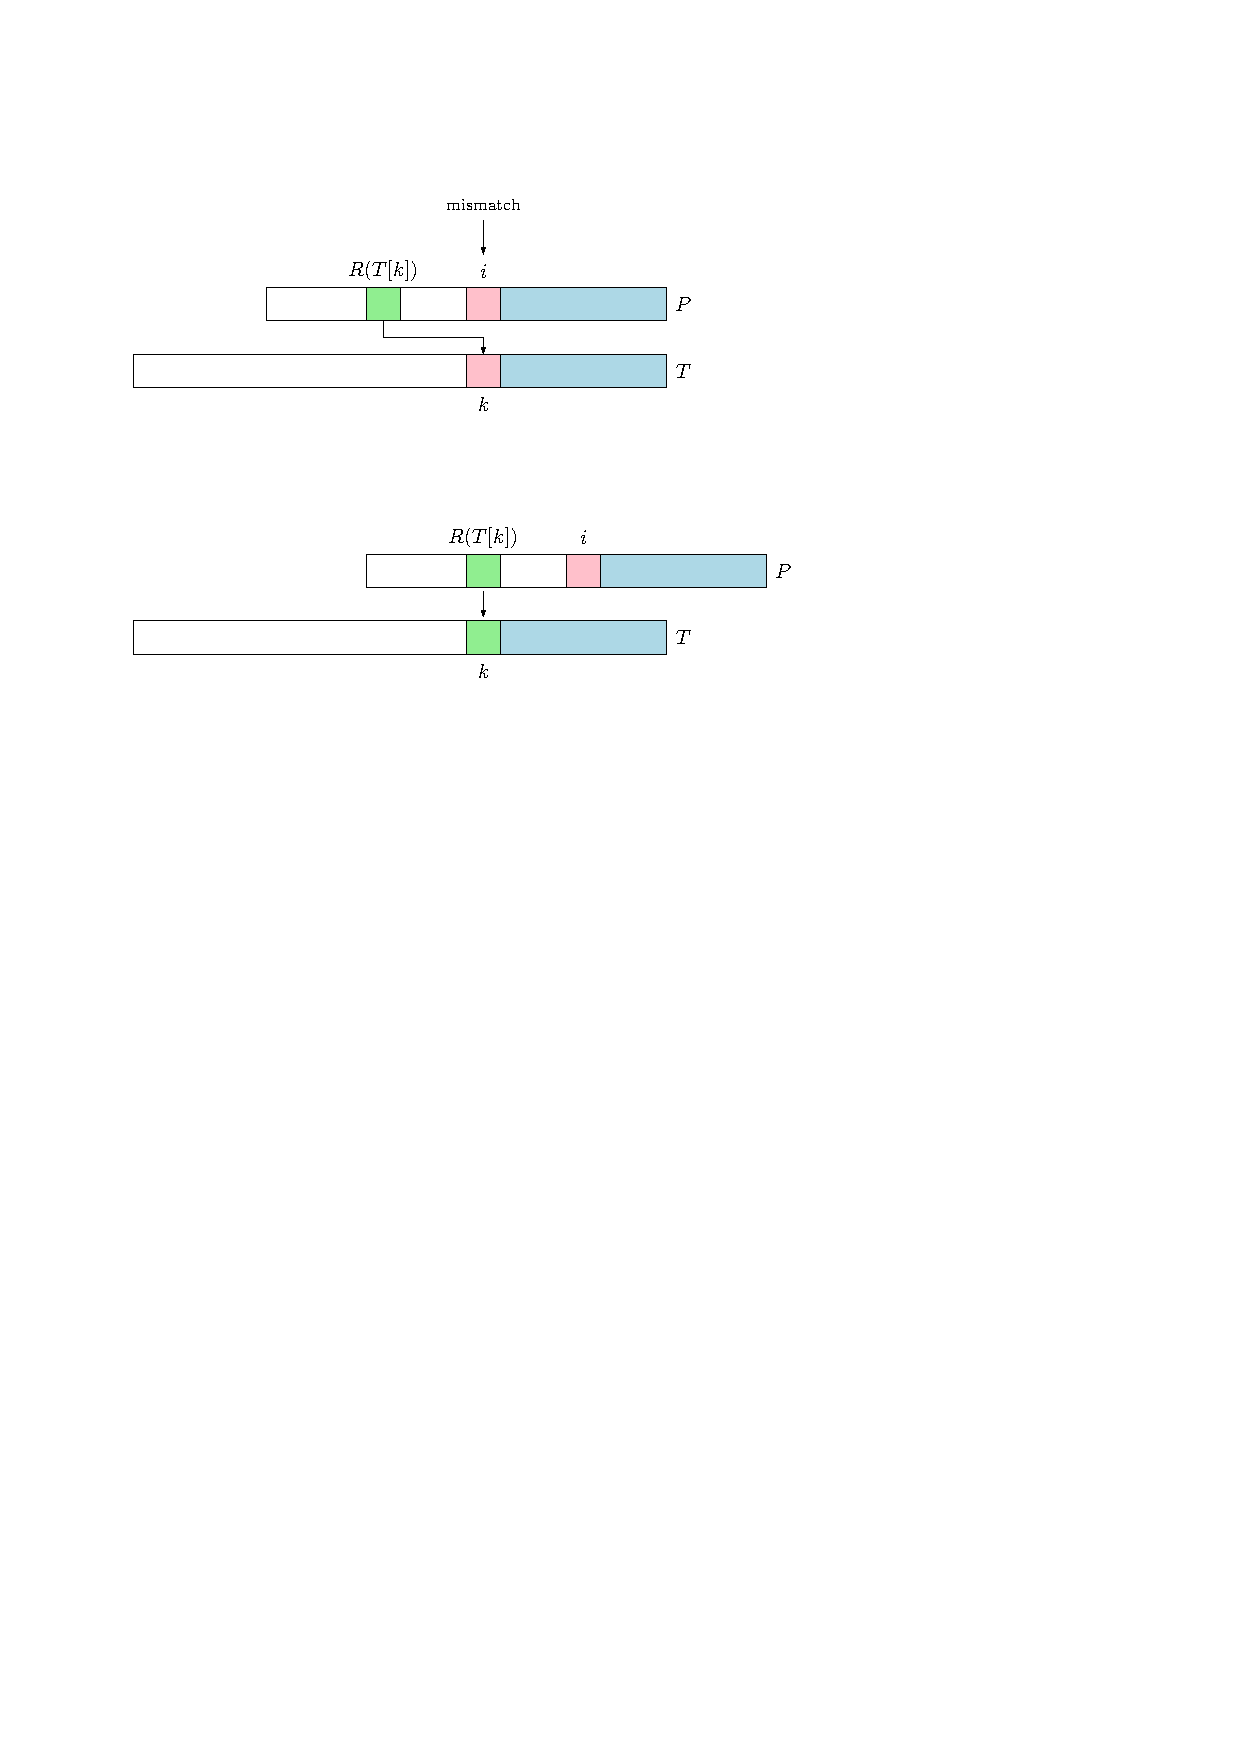
\includegraphics[width=0.8\linewidth]{boyer-moore/bad-character-rule.pdf}
    \caption{The bad character rule says to shift as much as possible so that a mismatch becomes a match.}
    \label{fig:boyer-moore-bad-char-rule}
\end{figure}

\subsection{Preprocessing for Bad Character Rule}

The bad character rule is quite straightforward to implement. In the preprocessing for the bad character rule, we find, for each position $i$ in the pattern $P$ and for each characther $x \in \Sigma$, the position of the closest occurrence of $x$ in $P$ to the left of $i$. This uses an $n \time \Sigma$ matrix. However, the time complexity for building this lookup table and the space required for it could be massive, depending on the length of the pattern and the size of the alphabet. It is also not hard to see that this approach can be quite space inefficient and we can end up store duplicate information over and over.

\begin{marginfigure}
    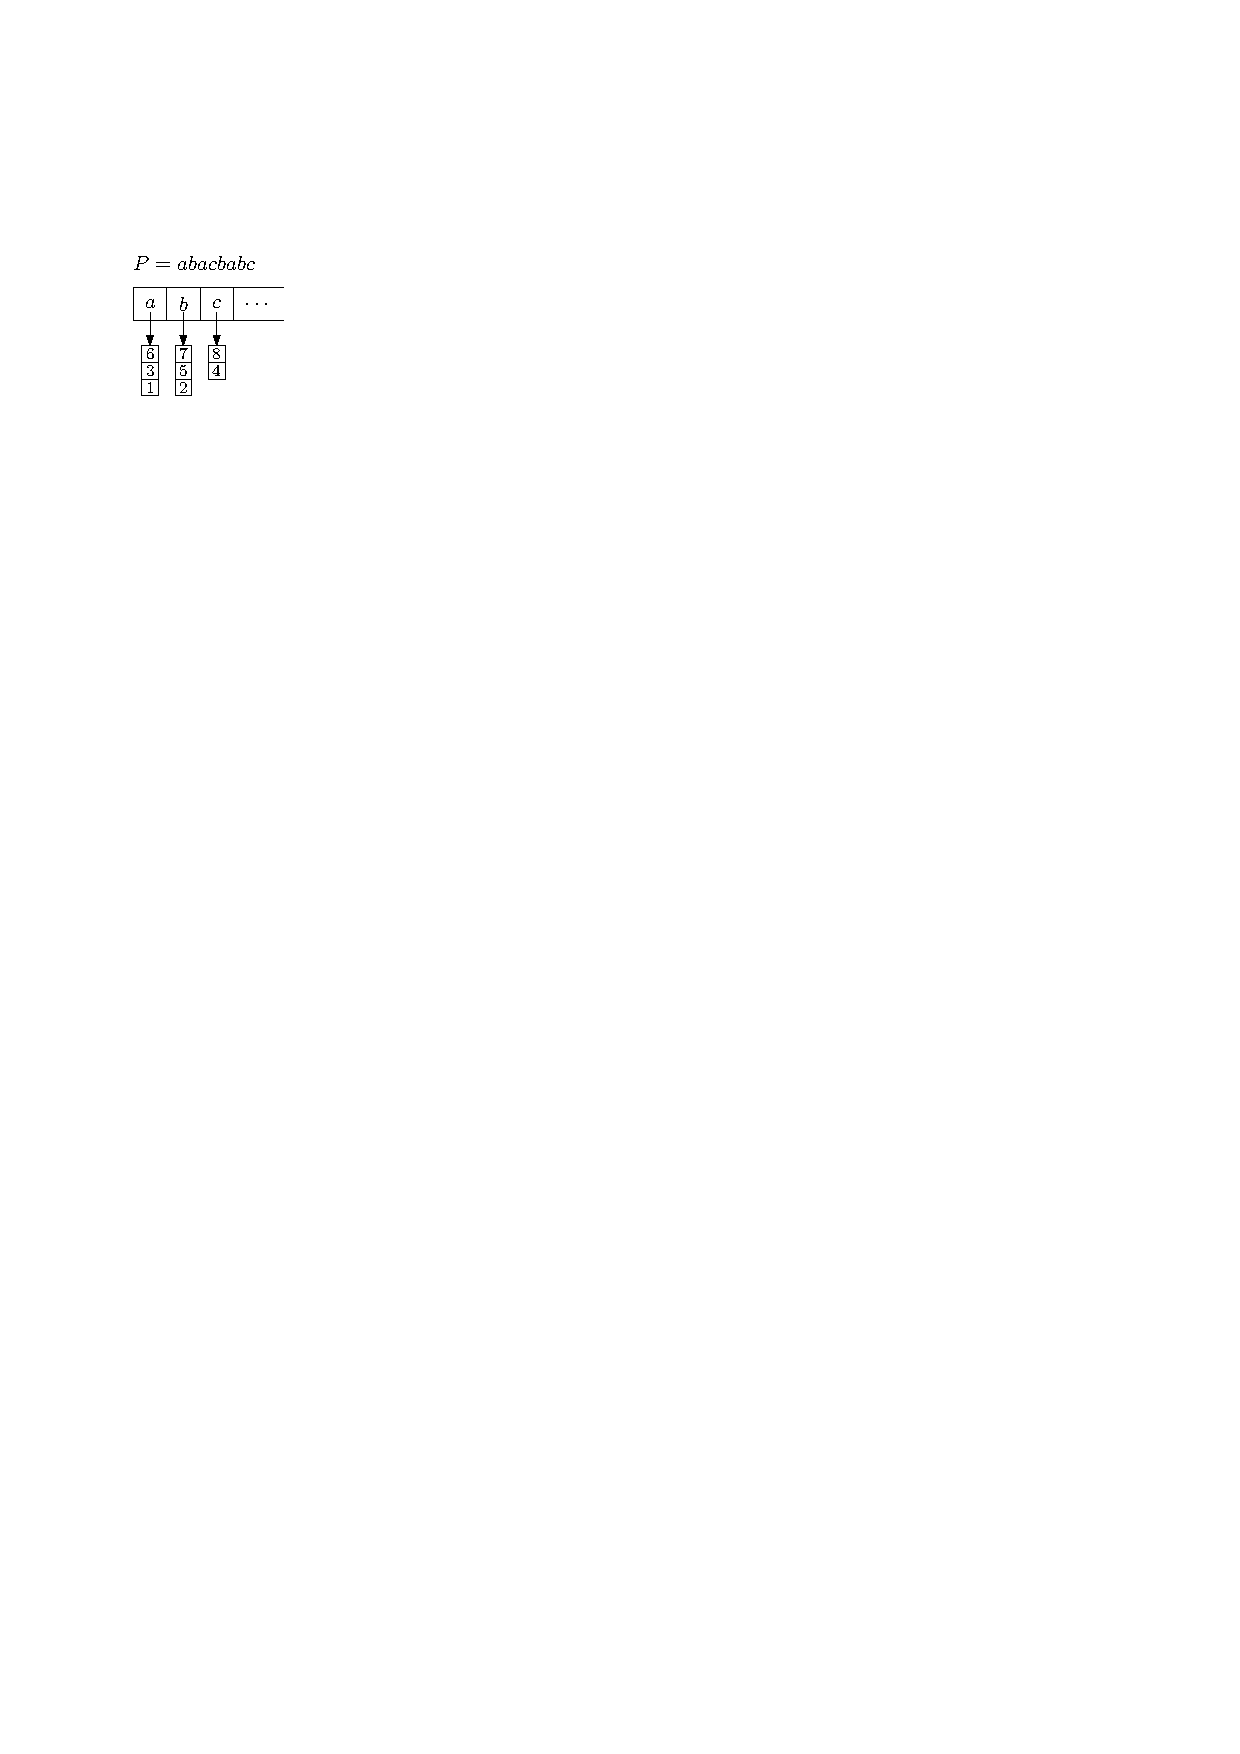
\includegraphics[width=0.5\linewidth]{boyer-moore/bad-character-rule-table.pdf}

    \hfill
    
    \caption{Table for storing information obtained from the bad character rule preprocessing.}
    \label{fig:bad-character-rule-table}
\end{marginfigure}

Alternatively, we can scan $P$ from right to left, and for each character $x \in \Sigma$, we keep a list of positions where $x$ occurs in $P$ (think hash table with chaining but just using another array instead of linked list). Since we scan $P$ from right to left, the indices will be stored in decreasing order for each character. It takes $O(n)$ space. During the actual execution of the Boyer-Moore algorithm, we can query this table whenever we need to find the rightmost occurrence of character $x$ left of index $i$. We can use \textit{binary search} for this.

If the alphabet $\Sigma$ is sparse, we can condense it by simply creating a mapping $f$ from $\Sigma \to \N$. The two approaches can be implemented as follows, respectively.

\begin{multicols}{2}
    \begin{codebox}
        \Procname{$\proc{Create-Bad-Char-Table}(P, f)$}
        \li $\id{table} = [\,]$
        \li $\id{row} = [0,\ldots,0]$
        \li \For $i = 1$ \To $|P|$ \Do
            \li $c = P[i]$
            \li $\id{table}.\proc{Append}(\id{row})$
            \li $\id{row}[f(c)] = i + 1$
        \End
        \li \Return $\id{table}$ 
    \end{codebox}
    
    \begin{codebox}
        \Procname{$\proc{Create-Bad-Char-Table}(P, f)$}
        \li $\id{table} = [\,]$
        \li \For $i = |P|$ \textbf{downto} $1$ \Do
            \li $c = P[i]$
            \li $\id{table}[f(c)].\proc{Append}(i)$
        \End
        \li \Return $\id{table}$ 
    \end{codebox}
    
\end{multicols}


\section{Good Suffix Rule}

\begin{rules}[Good Suffix Rule] \index{good suffix rule}
    \normalfont
    Given an alignment of $P$ against $T$, suppose a substring $t$ of $T$ matches a \textbf{suffix} of $P$, but a mismatch occurs at the next comparison to the left. Then, find, if exsits, the right-most copy $t'$ of $t$ in $P$ such that $t'$ is not a suffix of $P$. Shift $P$ to the right so that $t'$ in $P$ is matched with $t$ in $T$.
\end{rules}

Essentially, the \textit{\textbf{good suffix rule}} says we can shift as much as possible such that an \textit{existing match does not become a mismatch}. 

This rule is the weaker version of the good suffix rule used by Boyer and Moore's original publication. We now present a stronger version of the good suffix rule that allows us to prove properties of the Boyer-Moore algorithm more easily.

\section{Strong Good Suffix Rule}

\begin{rules}[Strong Good Suffix Rule] \index{strong good suffix rule}
    \normalfont
    Given an alignment of $P$ against $T$, suppose a substring $t$ of $T$ matches a \textbf{suffix} of $P$, but a mismatch occurs at the next comparison to the left. Then, find, if exsits, the right-most copy $t'$ of $t$ in $P$ such that $t'$ is not a suffix of $P$. Additionally, \textbf{we requires that the character left of $t'$ in $P$ differs from the character to the left of $t$ in $P$}. Shift $P$ to the right so that $t'$ in $P$ is matched with $t$ in $T$.
\end{rules}

\begin{figure}[htbp]
    \centering
    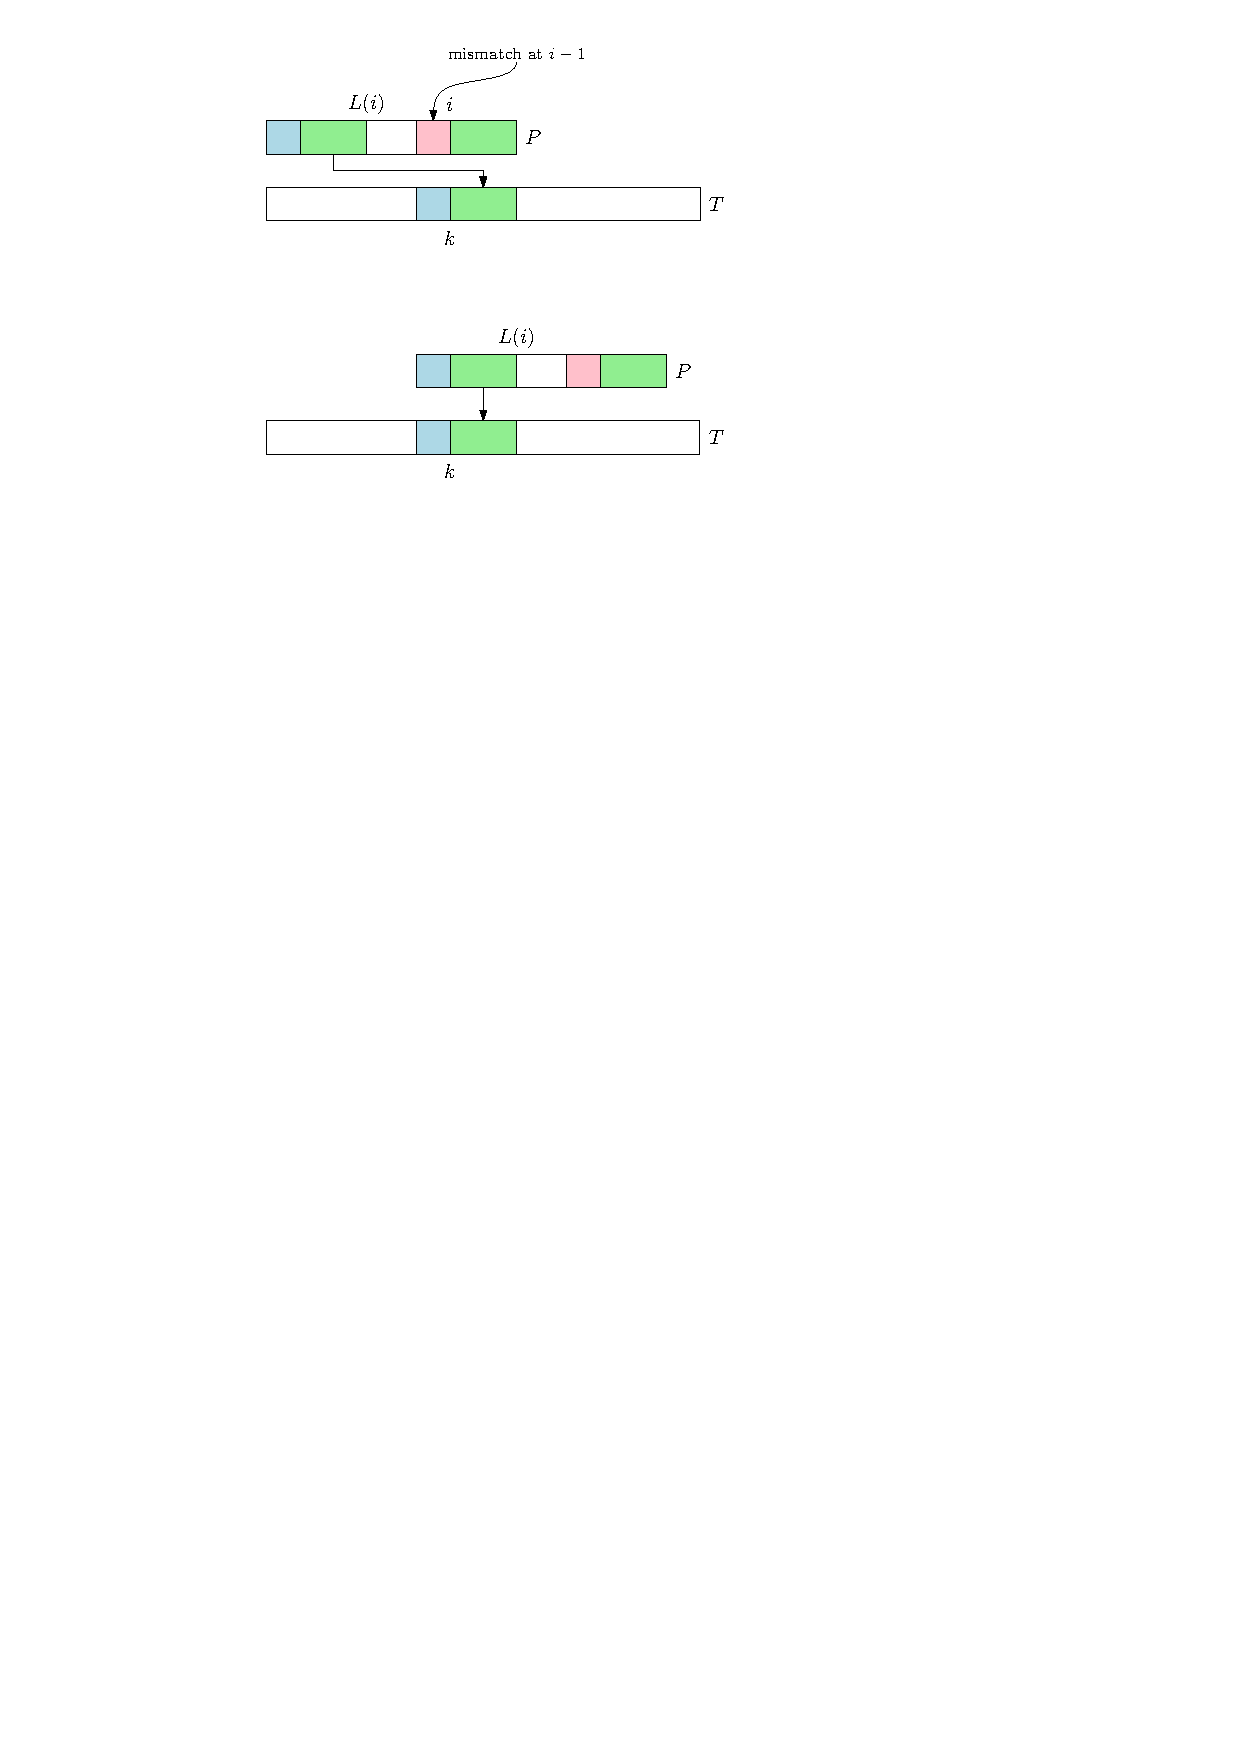
\includegraphics[width=0.6\linewidth]{boyer-moore/good-suffix-rule.pdf}
    \caption{The good suffix rule says we can shift as much as possible so long as a match does not become a mismatch. The additional requirement in the strong good suffix rule ensures that we don't encounter the same mismatch at $P[i-1]$.}
    \label{fig:boyer-moore-good-suffix-rule}
\end{figure}

Note the additional requirement stated in the second-to-last sentence. The addition of this requirement ensures that we don't get the same mismatch. A copy of $t$ is not worth looking at if it results in the same mismatch at the next character to the left. We call this rule the \textit{\textbf{strong good suffix rule}}. It should be obvious that it is safe to shift using the strong good suffix rule. That is, we won't miss any matches if we shift $P$ using the strong good suffix rule. We formalize this idea of correctness in the following theorem.

\begin{theorem}
    The strong good suffix rule does not shift $P$ past an occurrence in $T$.
\end{theorem}

\begin{proof}
    By contradiction. See Gusfield Theorem 2.2.1.
\end{proof}

\subsection{Preprocessing for Good Suffix Rule}


\begin{definition}
    For each $i$, let $L(i)$ be the \textbf{largest position} less than $n$ such that string $P[i\ldots n]$ matches a suffix of $P[1\ldots L(i)]$. If no such position exists, $L(i) = 0$.
    \begin{marginfigure}
        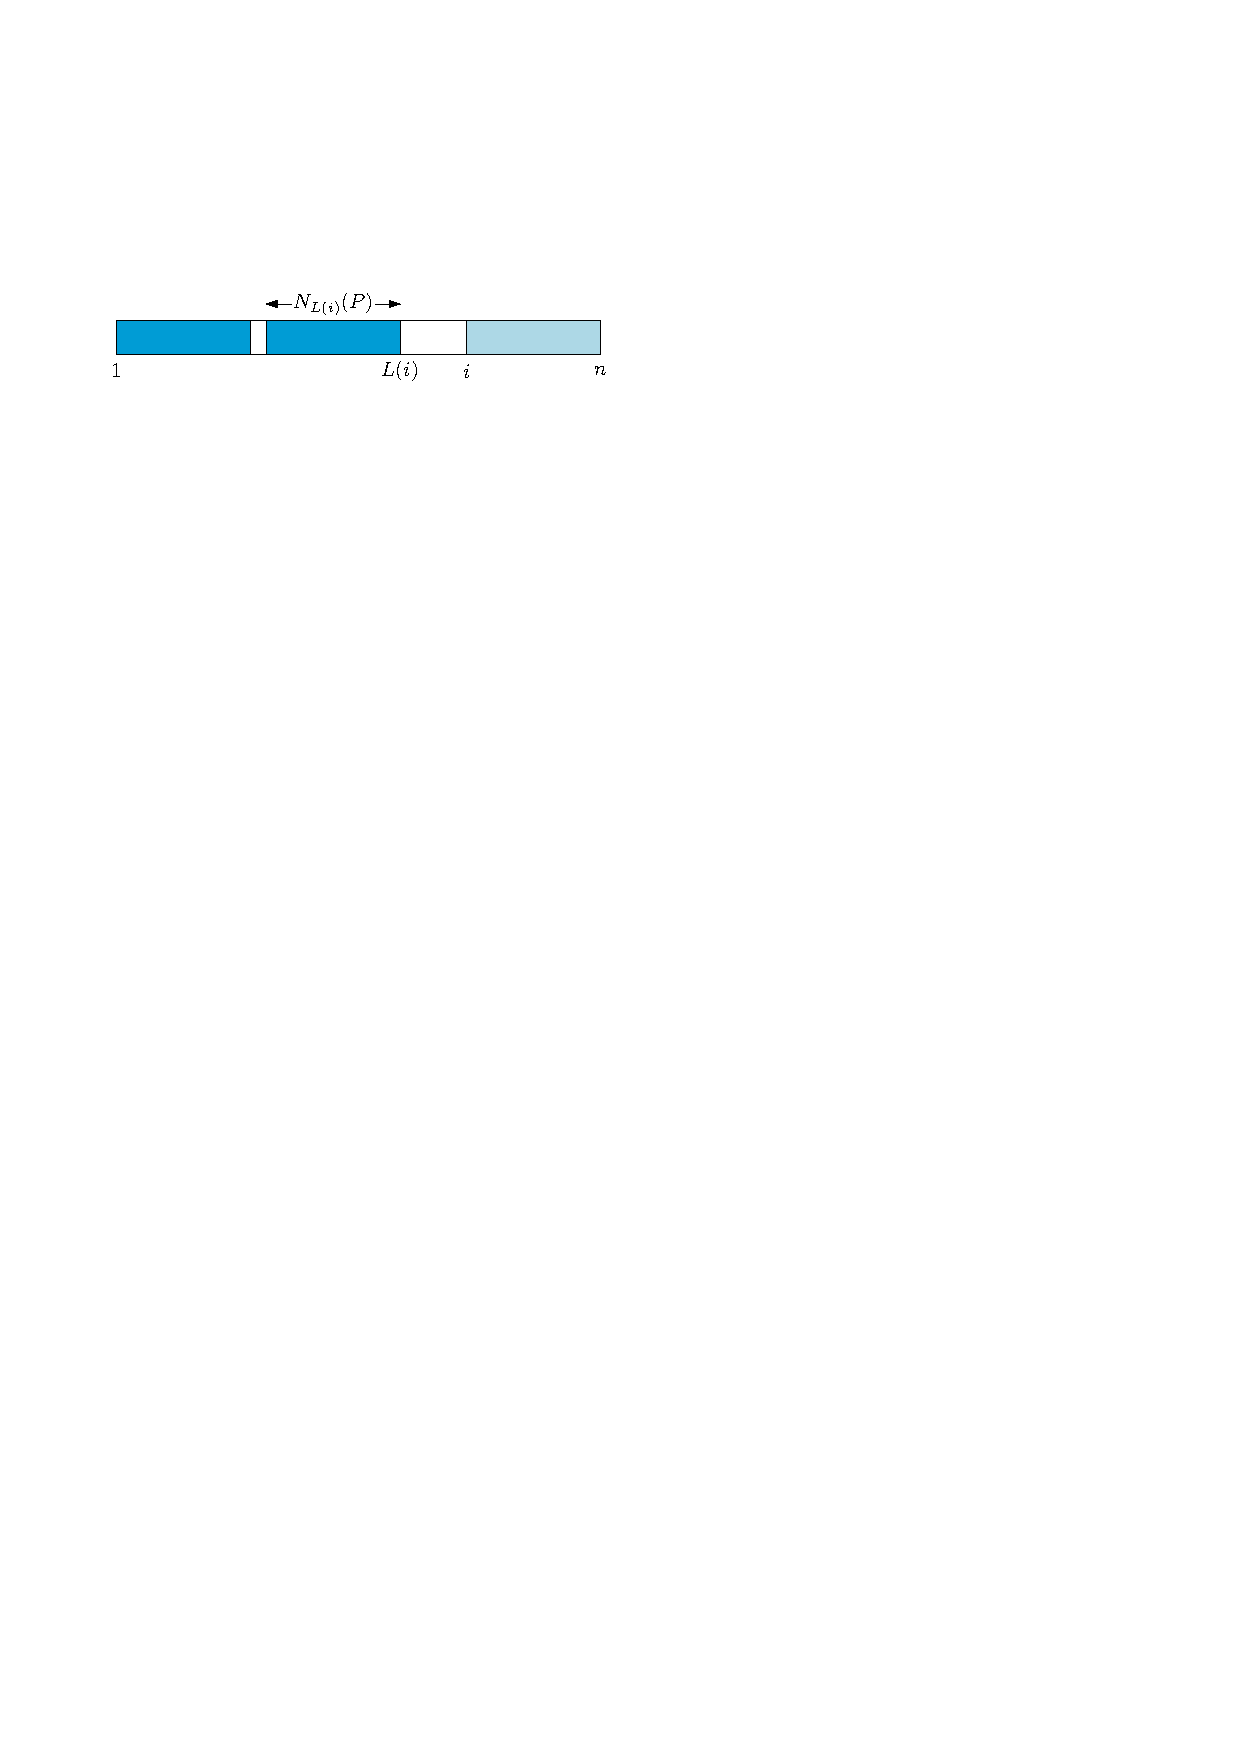
\includegraphics[width=\linewidth]{boyer-moore/good-suffix-Li.pdf}
        \caption{$L(i)$ gives the right-most copy of $t$ that is not a suffix of the whole string.}
        \label{fig:good-suffix-Li}
    \end{marginfigure}
    For each $i$, let $L'(i)$ be the largest position less than $n$ such that string $P[i \ldots n]$ matches a suffix of $P[1\ldots L'(i)]$ and such that the character preceding that suffix is not equal to $P[i-1]$. If no such position exists, $L'(i) = 0$.
\end{definition}

By definition, $L'(i)$ gives the right endpoint of the rightmost copy of $P[i\ldots n]$ that is not a suffix of $P$, and whose preceding character does not equal to $P[i-1]$.

\begin{definition}
    For string $P$, $N_j(P)$ is the length of the \textit{\textbf{longest suffix}} of the substring $P[1\ldots j]$ that is also a \textit{\textbf{suffix}} of the whole string $P$.
\end{definition}

\begin{theorem} \label{thm:good-suffix-Li-property}
    $L(i)$ is the largest index $j$ less than $n$ such that $N_j(P) \geq |P[i\ldots n]|$.
\end{theorem}

\begin{proof}
    By definition of $L$, $L(i)$ is the largest index less than $n$ such that $P[i\ldots n]$ matches a suffix of $P[1\ldots L(i)]$. 
    
    Let $j = L(i)$ in the definition of $N_j$. Then, $N_j(P)$ is the length of the longest suffix of the substring $P[1\ldots L(i)]$ that is also a suffix of the whole string. A suffix of the whole string must also be a suffix of $P[i\ldots n]$. Then, clearly, $N_j(P) \geq |P[i \ldots n]|$ because the substring $P[L(i)-N_j(P)+1 \ldots L(i)]$ can possibly match more characters left of $P[i]$.
\end{proof}

\begin{corollary}
    $L'(i)$ is the largest index $j$ less than $n$ such that $N_i(P) = |P[i\ldots n]| = n-i+1$.
\end{corollary}

\begin{proof}
    Immediate from Theorem \ref{thm:good-suffix-Li-property}. The definition requires that the characters left of $P[i]$ must not be contained in the suffix ending at $L'(i)$.
\end{proof}

One crucial observation is that $N_j$ is, in fact, the exact reverse of $Z_i$ when we talked about the Z-algorithm. Hence, $N_j(P)$ can be computed in linear time for all $j$ in linear time by calling \proc{Compute-Z} on $P^R$ (the reversal of $P$).

\begin{codebox}
    \Procname{$\proc{Compute-L'}(P)$}
    \li $N = \proc{Compute-Z}(P^R)$
    \li \For $i=1$ \To $|P|$ \Do
        \li $L'[i] = 0$ 
    \End
    \li \For $j = 1$ \To $|P|-1$ \Do
        \li $i = n - N[j] + 1$ 
        \li $L'[i] = j$ 
    \End
    \li \Return $L'$ 
\end{codebox}

\begin{definition}
    For string $P$, $l'(i)$ is the length of the \textit{\textbf{longest suffix}} of $P[i\ldots n]$ that is also a \textit{\textbf{prefix}} of the whole string $P$. If none exists, $l'(i)=0$.
    \begin{marginfigure}
        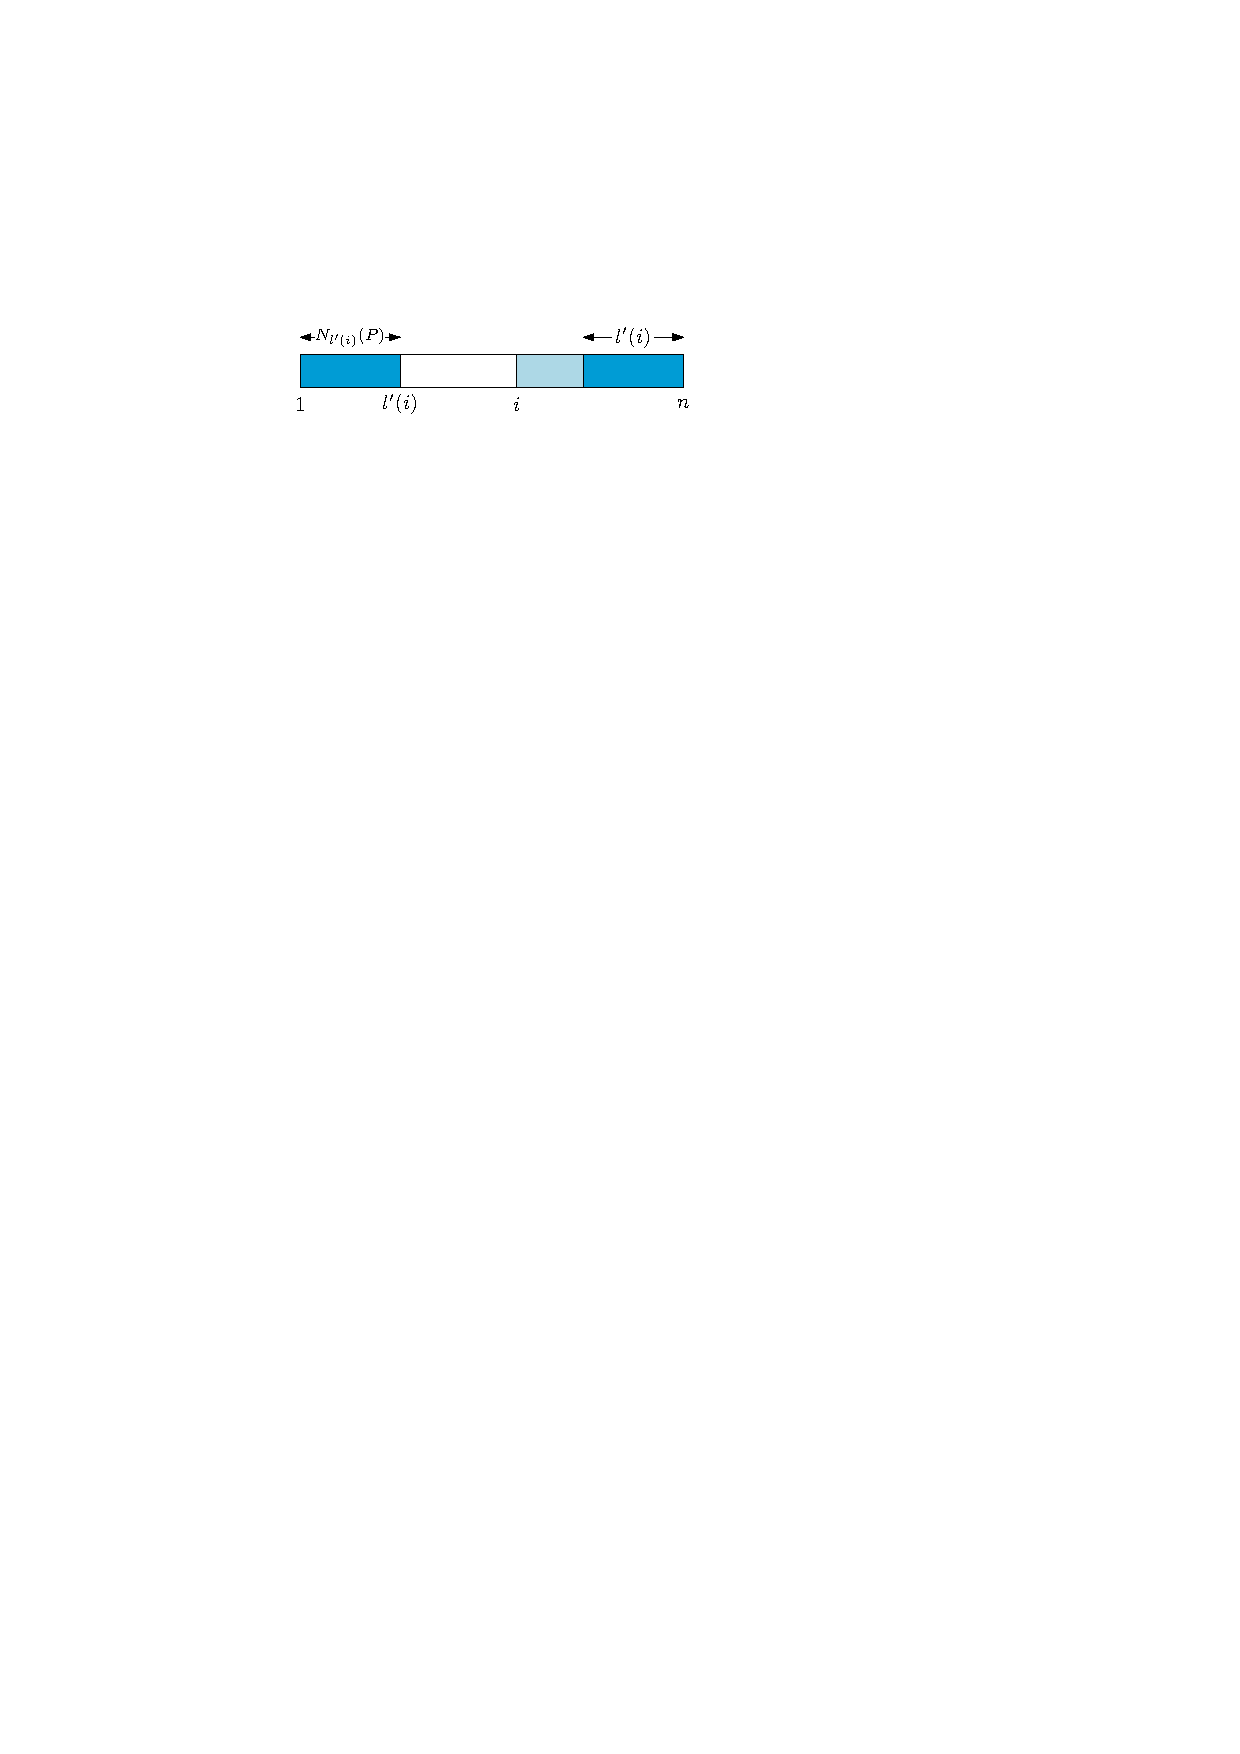
\includegraphics[width=\linewidth]{boyer-moore/good-suffix-ell-i.pdf}
        \caption{$l'(i)$ gives the index of the end of the longest prefix that matches a suffix of $P[i\ldots n]$.}
        \label{fig:good-suffix-ell-i}
    \end{marginfigure}
\end{definition}

\begin{theorem} \label{thm:good-suffix-ell-i-property}
    $l'(i)$ is the largest index $j \leq |P[i\ldots n]| = n-i+1$ such that $N_j(P)=j$.
\end{theorem}

\begin{proof}
    By definition of $l'$, the prefix $P[1\ldots l'(i)]$ is the longest prefix that matches a suffix of $P[i\ldots n]$. So $l'(i) \leq |P[i\ldots n]|$. A suffix of $P[i\ldots n]$ is also a suffix of $P$, so $P[1\ldots l'(i)]$ also matches a suffix of $P$.

    Let $j=l'(i)$ in the definition of $N_j$. Then, by definition of $N_j$, $P[l'(i)-N_{l'(i)}(P)+1\ldots l'(i)]$ is the longest suffix of $P[1\ldots l'(i)]$ that matches a suffix of $P$. The longest suffix of $P[1\ldots l'(i)]$ is $P[1\ldots l'(i)]$ itself, and indeed $P[1\ldots l'(i)]$ matches a suffix of $P$. Hence, $l'(i) = N_{l'(i)}(P)$. The maximality follows from the definition of $l'(i)$.
\end{proof}

\begin{codebox}
    \Procname{$\proc{Compute-$\ell'$}(P)$}
    \li $N = \proc{Compute-Z}(P^R)$
    \li \Comment{initialize $l'$ array}
    \li \For $i = 1$ \To $|P|$ \Do
        \li $l'[i] = 0$
    \End
    \li \Comment{set entires of $l'$ based on Theorem \ref{thm:good-suffix-ell-i-property}}
    \li \For $j = 1$ \To $|P|$ \Do
        \li \If $N[j] \isequal j$ \Then
            \li $l'[|P|-j+1] = j$
        \End
    \End
    \li \Comment{fill in $l'$ for $i$'s left of the longest suffix that matches a prefix}
    \li \For $i = |P|-1$ \textbf{downto} 1 \Do
        \li \If $l'[i] \isequal 0$ \Then
            \li $l'[i] = l'[i+1]$
        \End
    \End
    \li \Return $l'$ 
\end{codebox}

It may not be clear at first what the last for-loop on line 10-12 does. 
\begin{marginfigure}
    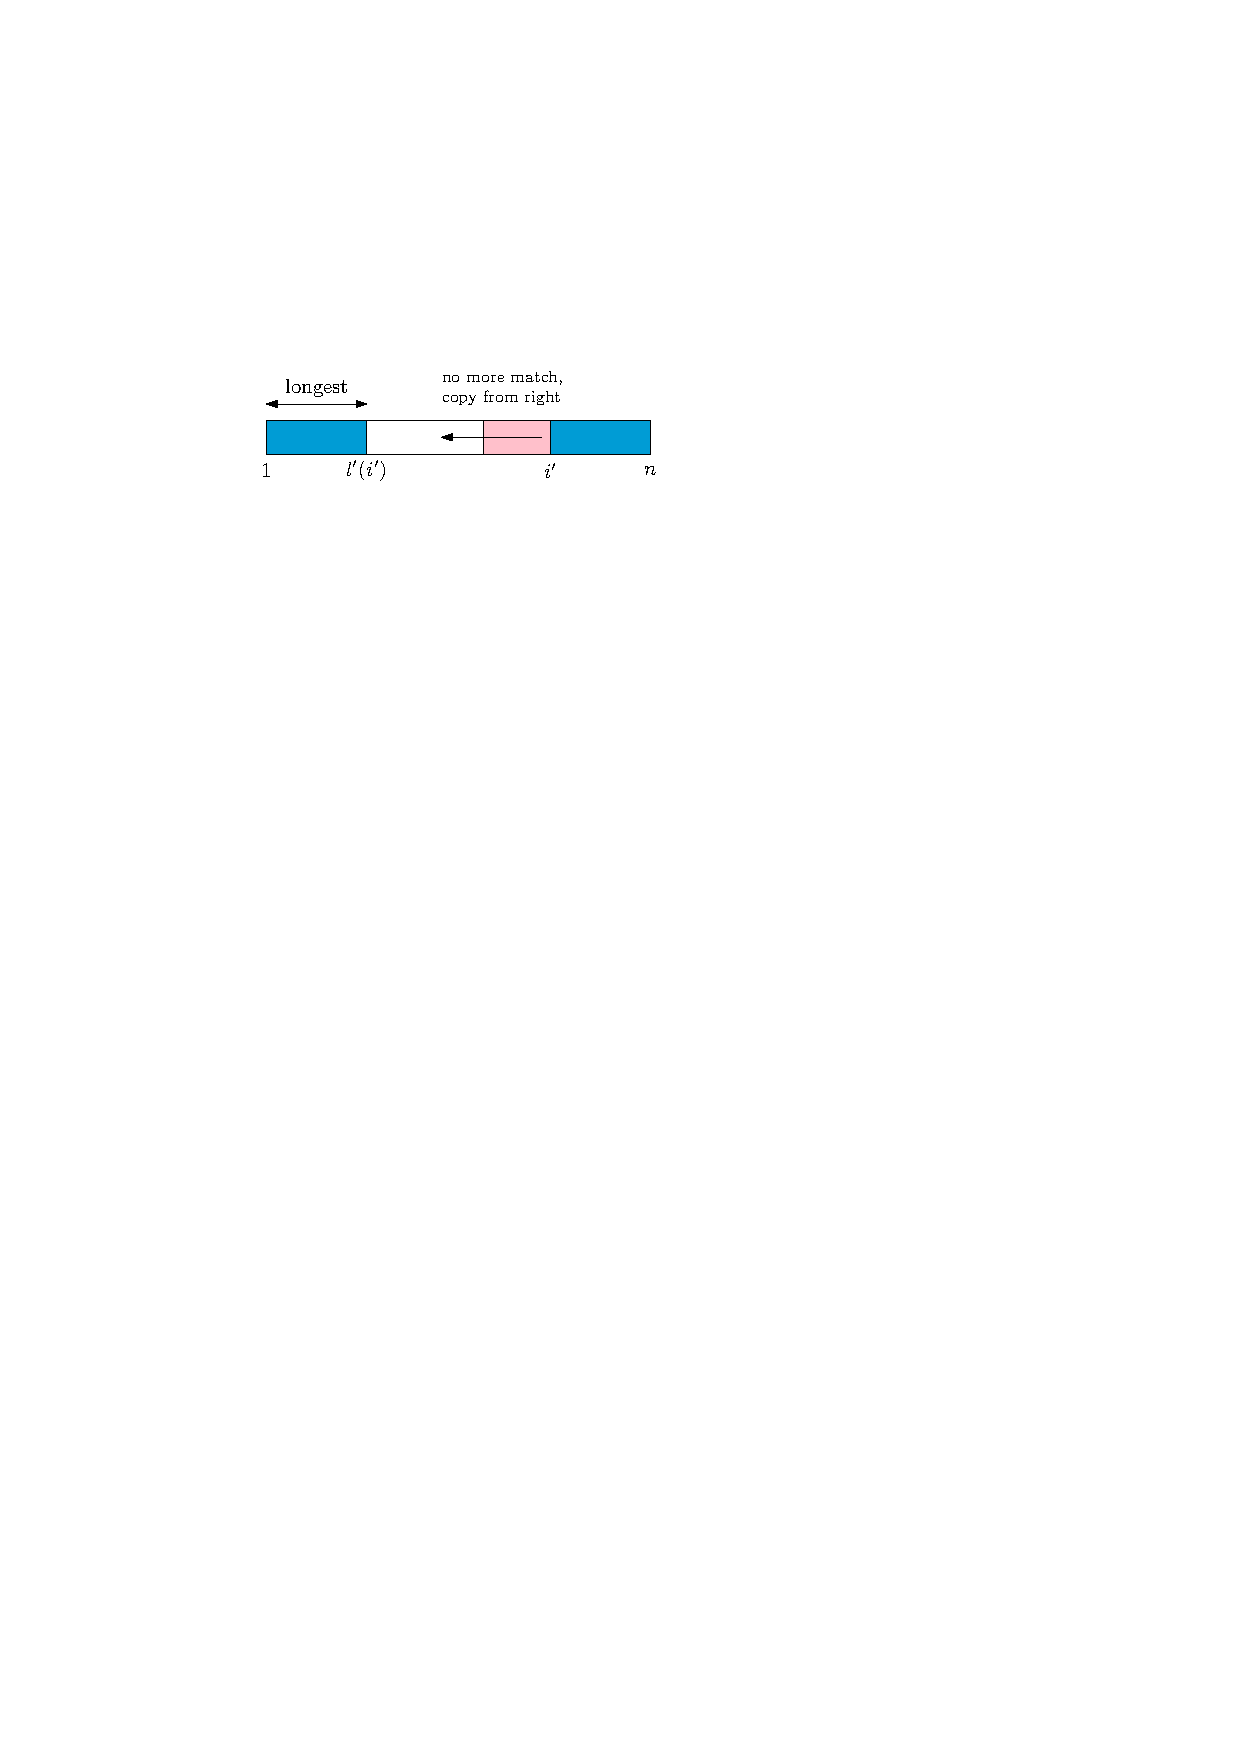
\includegraphics[width=\linewidth]{boyer-moore/good-suffix-ell-i-extension.pdf}
    \caption{``Smear'' to the left. This handles the cases when $P[i\ldots n]$ itself does not match a prefix of $P$, but some \textbf{proper suffix} $P[i' \ldots n]$ does.}
    \label{fig:good-suffix-ell-i-extension}
\end{marginfigure}
It copies the values of $l'$ from the right to fill in the blanks. Consider the example shown in Figure \ref{fig:good-suffix-ell-i-extension}. $P[1\ldots l'(i')]$ is the longest prefix that matches a suffix of $P$. For any $i < i'$, $P[i \ldots n]$ will not match a prefix of $P$. However, for those values of $i < i'$, $P[i'\ldots n]$ is \textbf{still a proper suffix} of $P[i \ldots n]$, so they ``inherit'' the $l'$ values from $l'(i')$ -- the left most position such that the entirety of $P[i'\ldots n]$ matches a prefix of $P$.

\section{Putting Everything Together}

\subsection{The Shifting Rules}

We summarize the shifting rules here. Remember that we are scanning from right to left.

\begin{enumerate}
    \item Bad character rule: Mismatch at $i$ with $T[k] \neq P[i]$; Shift $P$ to the right by $i - R(T[k])$.
    \item Good suffix rule: Mismatch at $i$ with $T[k] \neq P[i]$ but the suffix $P[i+1 \ldots n]$ matches some substring of $T$
    \begin{enumerate}
        \item If $L'(i) > 0$, then shift $P$ to the right by $n - L'(i)$
        \item If $L'(i) = 0$, then shift $P$ to the right by $n - l'(i)$ 
    \end{enumerate}
    \item No mismatch and $P$ is entirely matched with some substring of $T$, apply good suffix rule and shift $P$ to the right by $n - l'(2)$.
\end{enumerate}

\begin{figure}[htbp]
    \centering
    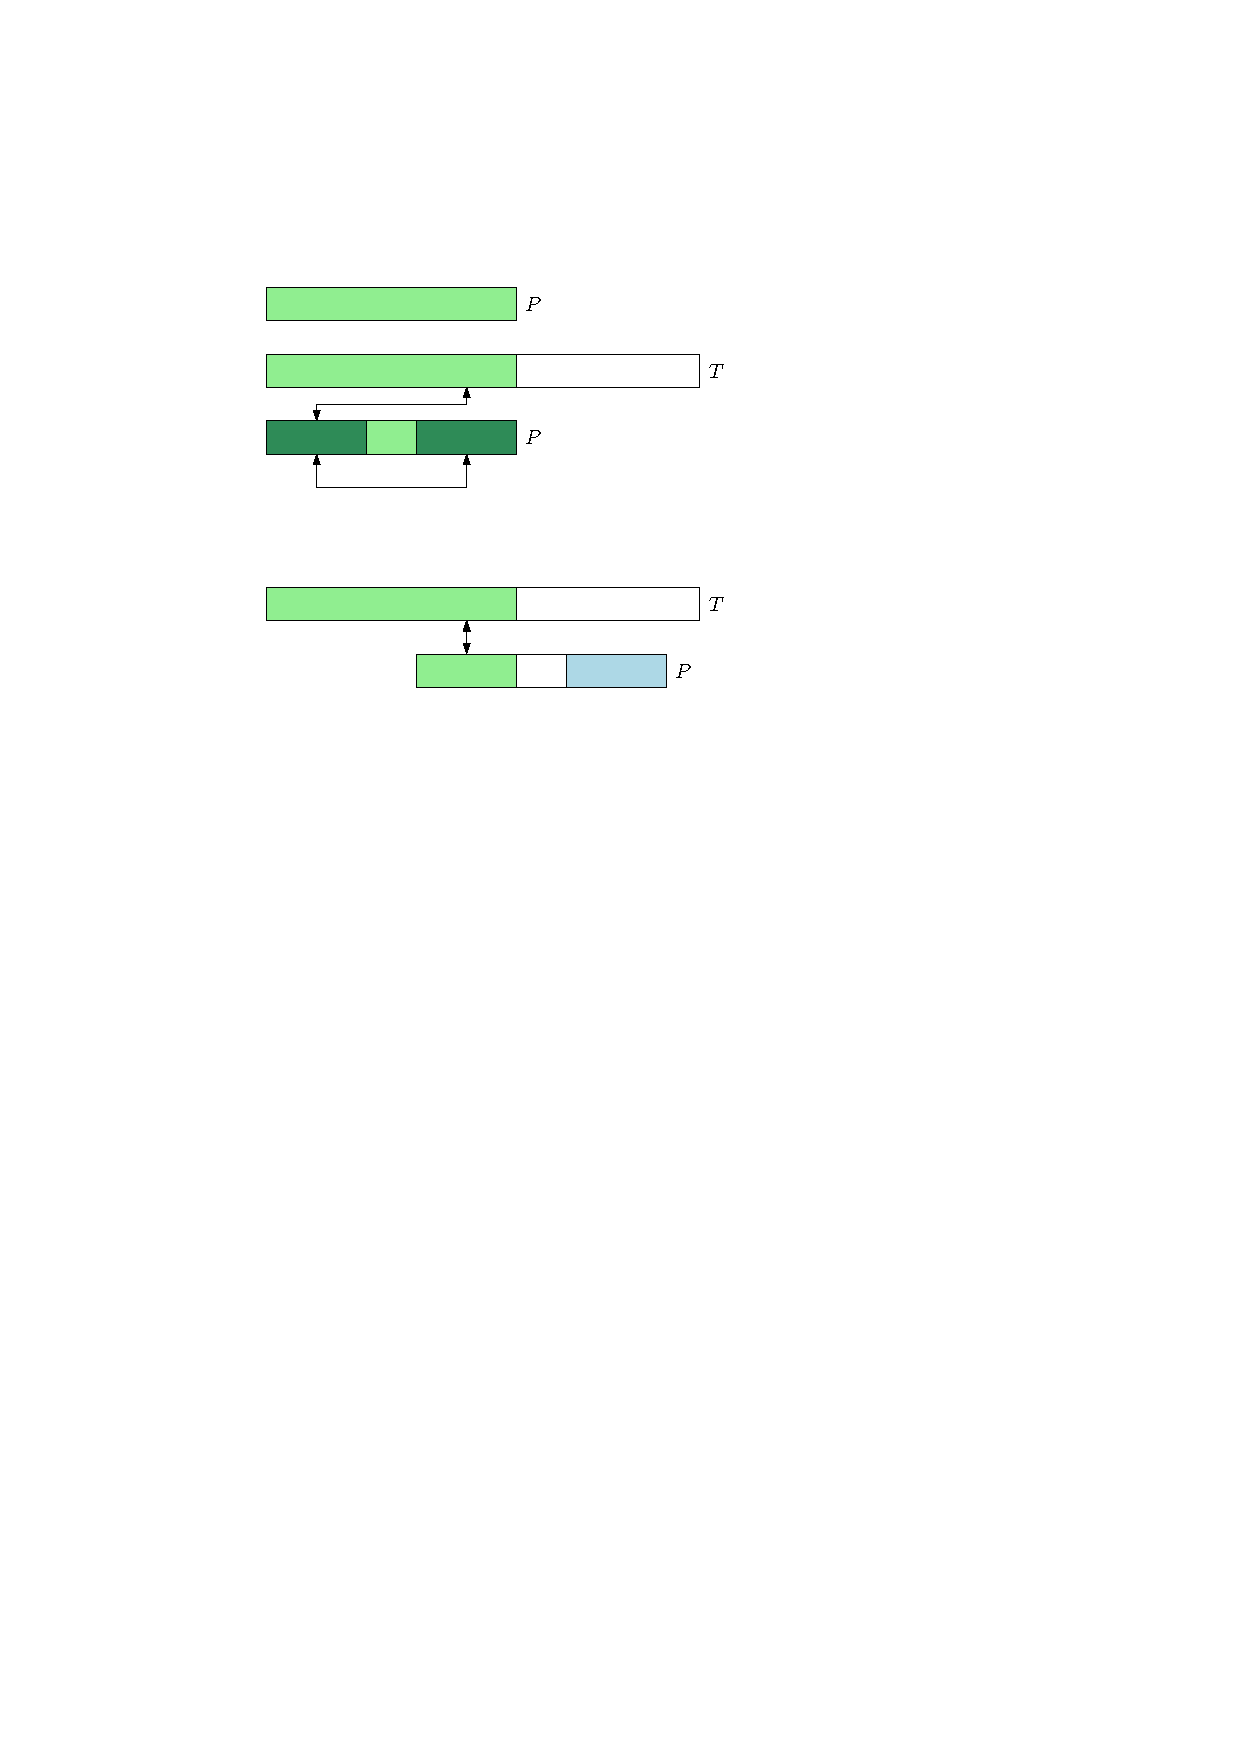
\includegraphics[width=0.6\linewidth]{boyer-moore/good-suffix-rule-full-match.pdf}
    \caption{The special good suffix rule when $P$ matches with $T$. We shift $P$ to the right so that a prefix of $P$ remains matched with $T$, if exists.}
    \label{fig:boyer-moore-good-suffix-rule-full-match}
\end{figure}

\subsection{Implementation}

For simplicity sake, we use $I$, the identity function when creating the bad character table. Again, in practice, if we are dealing with a sparse alphabet, we may want to change it to something else.

\begin{codebox}
    \Procname{$\proc{Boyer-Moore}(P,T)$}
    \li $L' = \proc{Compute-L'}(P)$
    \li $l' = \proc{Compute-$\ell'$}(P)$
    \li $R = \proc{Create-Bad-Character-Table}(P,I)$
    \li $k = |P|$
    \li \While $k \leq |T|$ \Do
        \li $i = n,\; h = k$
        \li \While $i > 0$ and $P[i] \isequal P[h]$ \Do
            \li $i = i - 1$
            \li $h = h - 1$
        \End
        \li \If $i = 0$ \Then
            \li $P$ found at position $h$ in $T$
            \li $k = k + |P| - l'[2]$
        \li \Else
            \li $\id{bc} = i - R[T[h]]$
            \li $\id{gs} = |P| - L'[i]$
            \li \If $\id{gs} \isequal 0$ \Then
                \li $\id{gs} = |P| - l'[i]$
            \End
            \li $k = k + \max\{\id{bc},\id{gs}\}$
\end{codebox}

\chapter{Knuth-Morris-Pratt Algorithm}

\part{Suffix Trees}

\chapter{Suffix Trees}
\section{Suffix Tries}

Let us recall the definition of a suffix.

\begin{definition}[Suffix] \index{suffix}
    For any string $S$, $S[i\ldots j]$ is the \textit{\textbf{substring}} starting at position $i$ and ending at position $j$; $S[1\ldots i]$ is the prefix of $S$ ending at $i$; and $S[j\ldots |S|]$ is the \textit{\textbf{suffix}} of $S$ starting at position $j$. A proper substring, prefix, or suffix is a substring, prefix, or suffix that is neither the entire string $S$ nor the empty string.
\end{definition}

Then, we define a trie and a suffix trie as follows.

\begin{definition}[Suffix Trie] \index{trie} \index{suffix trie}
    A \textit{\textbf{trie}} is the smallest tree such that each edge is labeled with a character from the alphabet $\Sigma$, each node has at most one outgoing edge labeled with $c$ for each $c \in \Sigma$, and each node has a key that is the concatenation of the edge labels along the path from the root to that node. A \textit{\textbf{suffix trie}} is a trie where each root-to-leaf path represents a suffix.
\end{definition}

\begin{figure}[htbp]
    \centering
    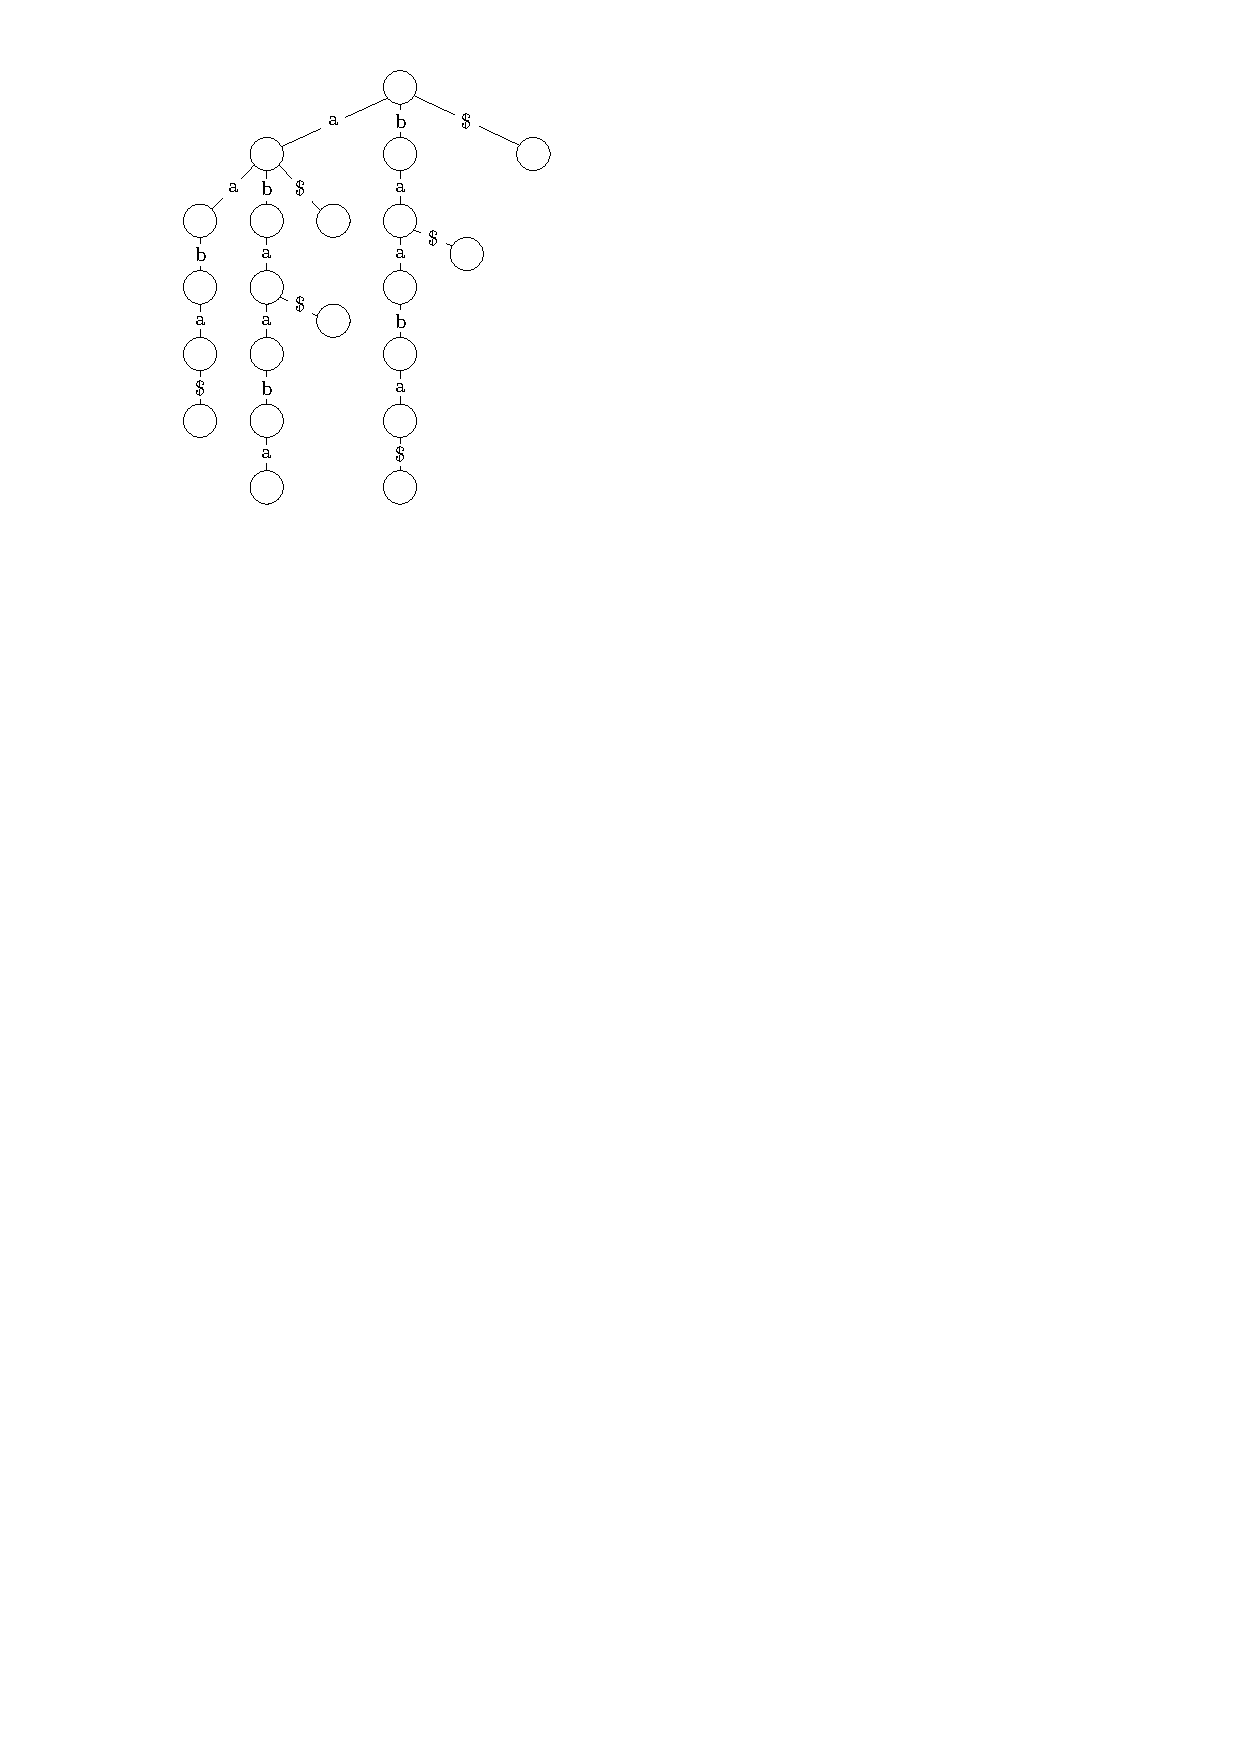
\includegraphics[width=0.45\linewidth]{suffix-tree/suffix-trie.pdf}
    \qquad
    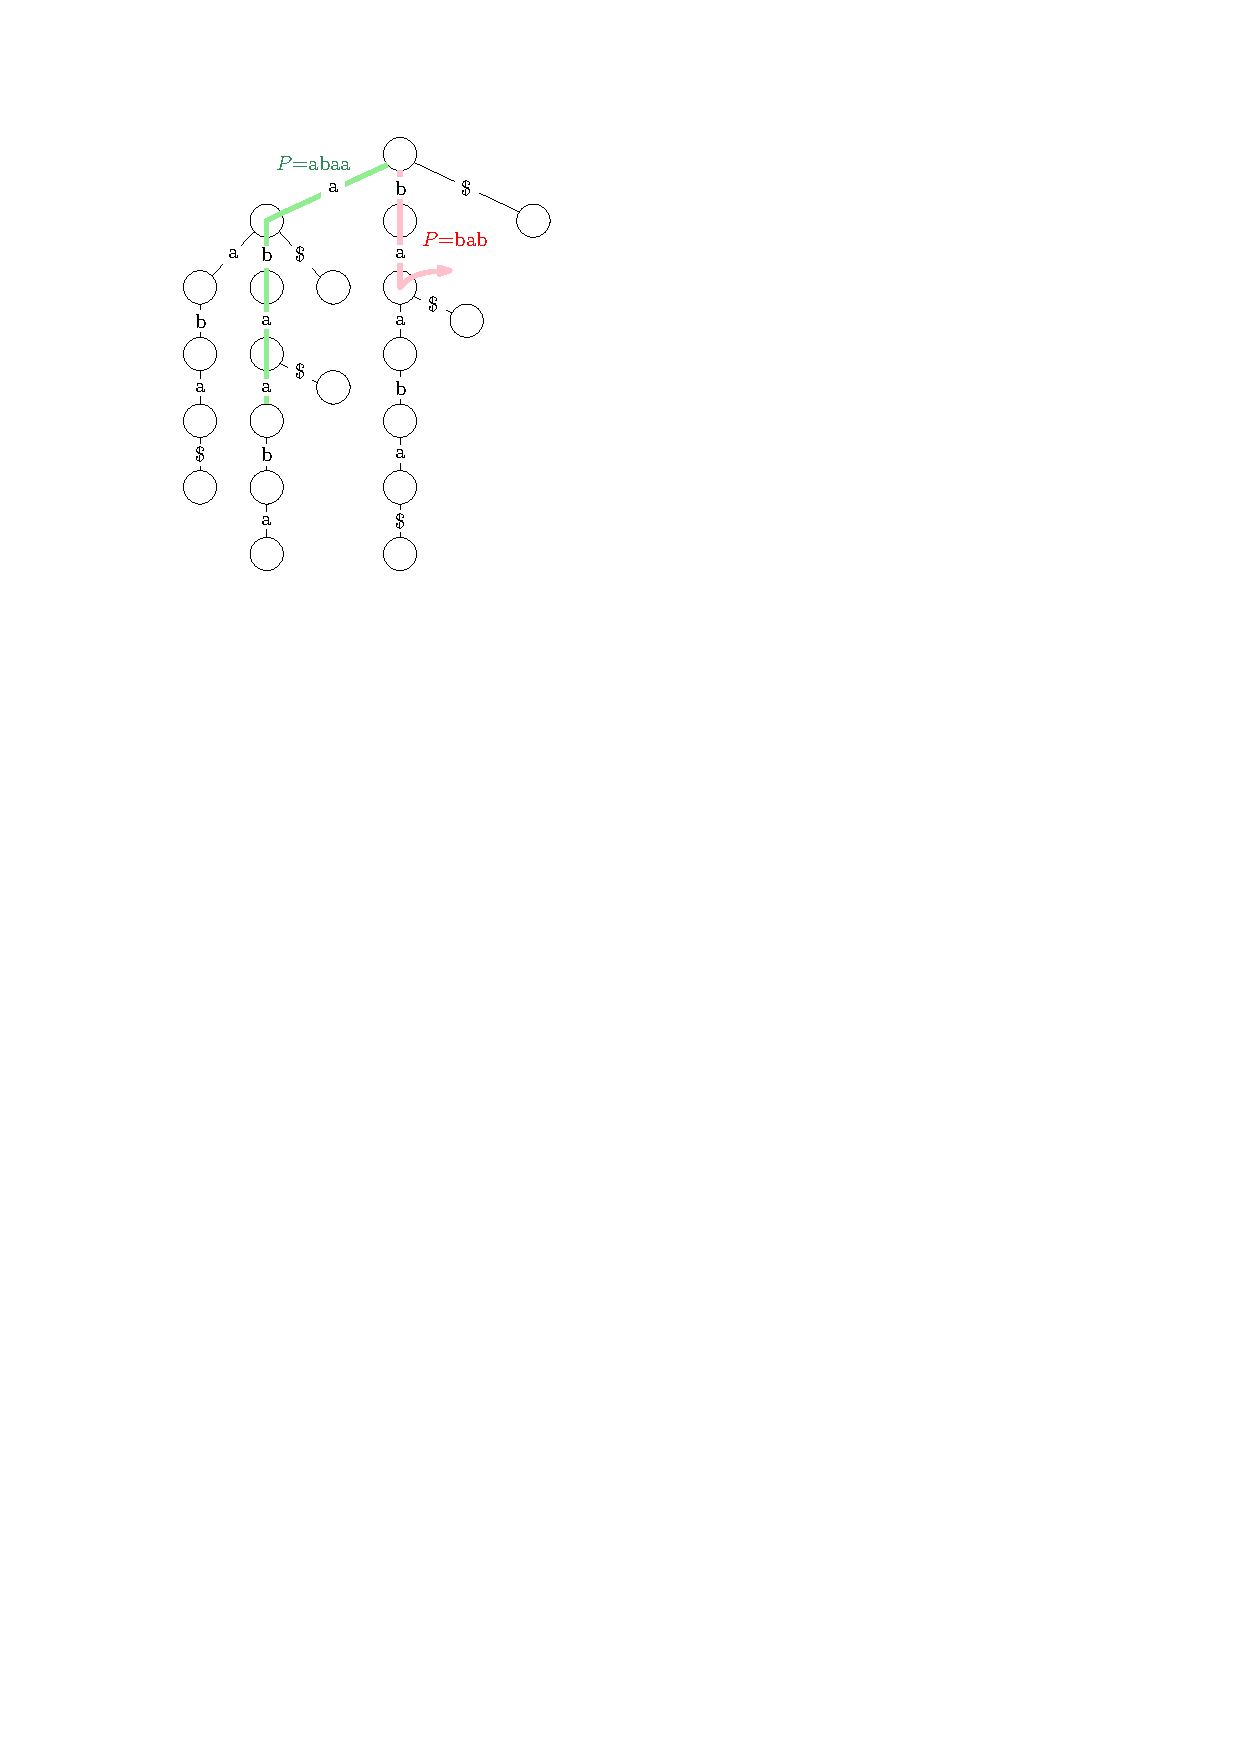
\includegraphics[width=0.45\linewidth]{suffix-tree/suffix-trie-search-path.pdf}
    \caption{Suffix trie for $T = abaaba$. On the right: the search path for $P=abaa$ and $P=bab$. When searching for a pattern that is not in $T$, we ``fall off'' the trie.}
    \label{fig:suffix-trie}
\end{figure}

In a regular tree (e.g. binary search tree), the key is stored at each node. In a trie, the keys are \textit{implicitly} represented by the edge labels along the path. Figure \ref{fig:suffix-trie} shows a suffix trie constructed for $T = abaaba$.

It is important to add the terminator character \texttt{\$} at the end of the string. If we remove the terminator \texttt{\$}, it is not hard to see the result trie may no longer be a valid suffix trie. We assume that \texttt{\$} is \textit{lexicographically smaller than all characters} in $\Sigma$.

\subsection{Search in Suffix Trie}

\newthought{Search for Pattern}: It is easy to search for a pattern $P$ given a suffix trie. We can \textbf{start from the root and follow the edges labeled with the characters} in $P$ until we either finish reading the pattern and find a match, or ``fall off'' the trie, in which case we can return that a match is not found.

\begin{codebox}
    \Procname{$\proc{Search-Trie}(P,T)$}
    \li $\id{cur} = \attrib{T}{\id{root}}$
    \li \For $c$ \textbf{in} $P$ \Do
        \li \If $c \not\in \attrib{\id{cur}}{edges}$ \Then
            \li \Return \const{false}
        \li \Else $\id{cur} = \attrib{\id{cur}}{edges}[c]$
        \End
    \End
    \li \Return $\id{cur} \neq \const{null}$ 
\end{codebox}

Assume that at each node, we maintain a hash table for each outgoing edges. Then, the algorithms runs in expected time $\Theta(|P|)$.

\newthought{Search for Suffix}: Similarly, if we want to see if a given pattern $P$ is a suffix of $T$, we can run the same algorithm and checks if the node at the end of the path has an outgoing edge labeled \texttt{\$}.

\newthought{Search for Number of Occurrences}: If we are interested in the number a pattern $P$ occurs as a substring in $T$, we can run \proc{Search-Trie}. Once we arrive at the end of our search path, we run a \textbf{depth-first search} from the node at the end of the search path and count the number of leaf nodes reachable from that node. Since a trie is a tree, DFS runs in $O(|V|)$ time. In this case, it takes $O(|P|+|T|)$ time to find the number of occurrences of a given pattern.

\textsc{Search for Longest Repeated Substring}: Find the deepest (internal) node with more than one children.

\subsection{Space Complexity of Suffix Trie}

\begin{marginfigure}
    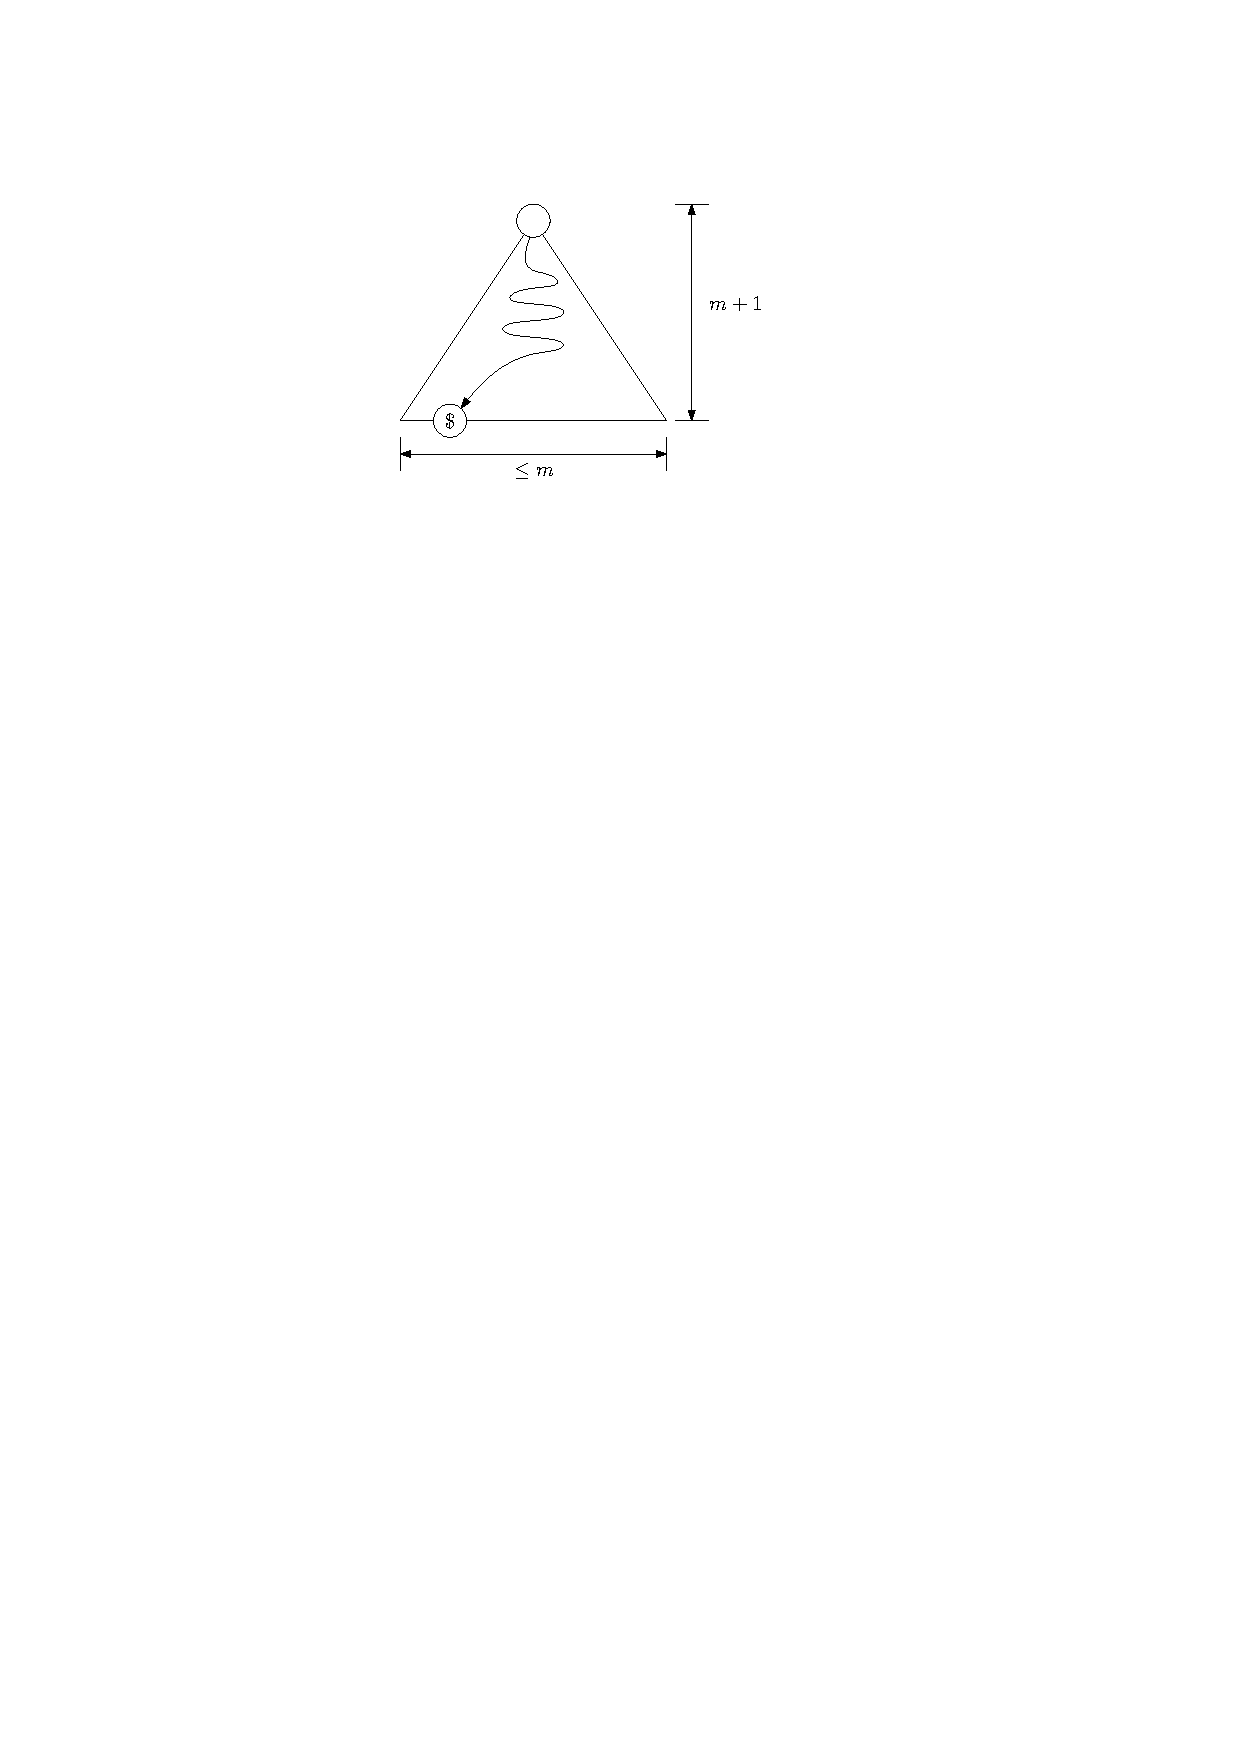
\includegraphics[width=\linewidth]{suffix-tree/suffix-trie-size.pdf}
    \caption{Max width and height of a suffix trie. The path from the root to the deepest leaf represents the longest suffix (the whole string plus the terminator).}
\end{marginfigure}

\subsection{Construct a Suffix Trie}

\section{Suffix Tree}

\subsection{From Suffix Trie to Suffix Tree}


\chapter{Constructing Suffix Trees}

\part{Dynamic Programming}

\chapter{Edit Distance}

\part{Compression and Indexing}

\chapter{Entropy and Information}

\chapter{k-mer Index and Suffix Array}
\section{Idea Behind Indexing}

Suppose you have a textbook and you want to look for a certain term, say, the word ``\textit{string}''. It would be really time-consuming, and in some cases, impossible to look for the term by going through the book page by page. That's why most books usually (and hopefully) have an index at the end, which list the pages where each term occurs.

\begin{figure}
    \centering
    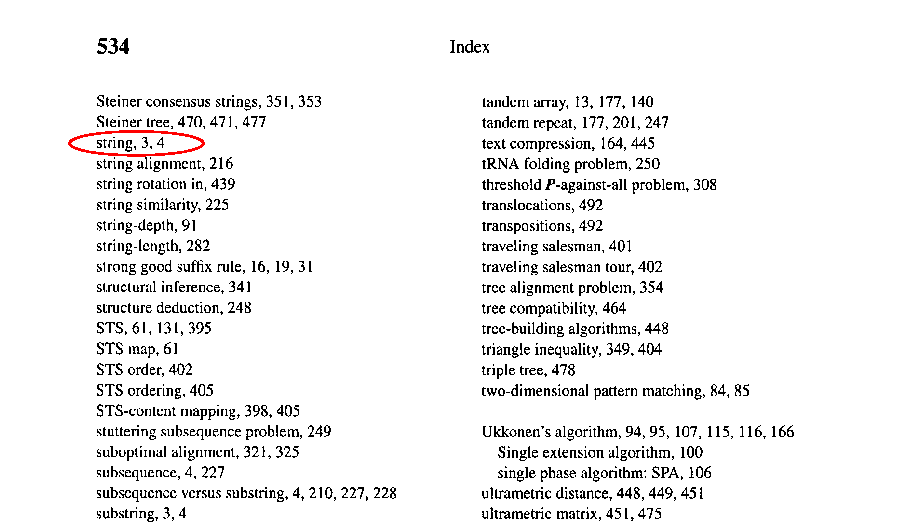
\includegraphics[width=\linewidth]{index/example-gusfield-idx.pdf}
    \label{fig:example-gusfield-idx}
    \caption{The index of Gusfield's textbook, with the term ``string'' circled.}
\end{figure}

Index can help us speed up query speed and also give us a compact representation of the data.

Two big ideas behind indexing are \textit{\textbf{grouping}} and \textit{\textbf{ordering}}. The first index that we will look at, $k$-mer index, uses grouping.

\section{\textit{k}-mer Index}

Given a text $T$, we call all its substrings of length $k$, the \textit{\textbf{k-mers}} of $T$. For example, consider the string \texttt{CGTGCGTGCTT}, it has the following 5-mers: \texttt{CGTGC}, \texttt{GCGTG}, \texttt{GTGCC}, \texttt{GTGCT}, \texttt{TGCCT}, and \texttt{TGCTT}. The substrings \textit{can have overlaps}.

$k$-mer index groups the indices of $T$ by the $k$-mer that starts at the index. So, for the string \texttt{CGTGCGTGCTT}, we have the $k$-mer index for $k=5$:

\begin{table}
    \centering
    \begin{tabular}[H]{c|c}
        $k$-mer & indices \\
        \hline
        \texttt{CGTGC} & 0, 4 \\
        \texttt{GCGTG} & 3 \\
        \texttt{GTGCC} & 1 \\
        \texttt{GTGCT} & 5 \\
        \texttt{TGCCT} & 2 \\
        \texttt{TGCTT} & 6
    \end{tabular}
\end{table}

It is easy to construct a $k$-mer index. We can scan the string from left to right and record the position of each $k$-mer. It takes $|T|-k+1$ time.

\section{Querying k-mer Index}

To query a $k$-mer index efficiently, we should first \textit{sort the index lexicographically} by the $k$-mers. It takes $k(|T|-k)\log(|T|-k) \in O(|T|^2 \log|T|)$ steps. To compare two $k$-mers, we need $k$ steps (unlike comparing two numbers or characters, which takes constant time), and sorting the list of $|T|-k$ $k$-mers takes $\Theta((|T|-k)\log(|T|-k))$. There is a bit of tradeoff here. If we choose a small $k$, we spend less time comparing two substrings during sorting, but we can possibly end with many $k$-mers in the list; in we choose a large $k$, it takes more time to compare two substrings, but we will have fewer $k$-mers to sort.

Once we sort the $k$-mer index, we can use \textit{binary search} for patterns $P$ such that $|P| \leq k$. It takes $O(|P|\log |T|)$ to query a sorted $k$-mer index. However, if $|P| > k$, $k$-mer index can be inefficient since we need to \textit{manually extend the match} once the first $k$ characters of $P$ matches a substring in $T$.

\chapter{Burrows-Wheeler Transform}

\chapter{FM Index}

\chapter{Wavelet Tree}

\backmatter

\bibliographystyle{abbrvnat}
\bibliography{stringbook}
\addcontentsline{toc}{chapter}{Bibliography}

\printindex

\end{document}

